\documentclass{article}

% NeurIPS 2024 / Preprint Styling
\usepackage[preprint]{neurips_2024}

\usepackage[utf8]{inputenc}
\usepackage[T1]{fontenc}
\usepackage{amsmath,amssymb,amsfonts,amsthm}
\usepackage{mathtools}
\usepackage{booktabs}
\usepackage{tabularx}
\usepackage{array}
\usepackage{algorithm}
\usepackage{algorithmic}
\usepackage{graphicx}
\usepackage{xcolor}
\usepackage{microtype}
\usepackage{url}
\usepackage{hyperref}
\usepackage[capitalise,noabbrev]{cleveref}
\usepackage{natbib}
\usepackage{enumitem}
\usepackage{multirow}
\usepackage{bm}

\hypersetup{
    colorlinks=true,
    linkcolor=blue!70!black,
    citecolor=blue!70!black,
    urlcolor=blue!70!black
}

% Mathematical Theorem Environments
\newtheorem{theorem}{Theorem}
\newtheorem{lemma}[theorem]{Lemma}
\newtheorem{proposition}[theorem]{Proposition}
\newtheorem{corollary}[theorem]{Corollary}
\theoremstyle{definition}
\newtheorem{definition}{Definition}
\newtheorem{remark}{Remark}

\title{\textbf{Ligand Fingerprints, Not Expert Routing or Pocket Conditioning, Drive Cross-Family Affinity Prediction in Protein Foundation Models: A Controlled Study on 56,637 Measured ChEMBL Records}}

\author{
  \textbf{Md Mushfiqur Rahim}\thanks{Correspondence: \texttt{20mahin2020@gmail.com} \quad ORCID: \href{https://orcid.org/0009-0003-1021-685X}{0009-0003-1021-685X} \quad GitHub: \href{https://github.com/MD-Mushfiqur123}{MD-Mushfiqur123} \quad Prior Work DOI: \href{https://doi.org/10.5281/zenodo.23841930}{10.5281/zenodo.23841930}} \\
  Independent Researcher \quad \textit{Clinical Neuroscience \& AI Systems Architecture}
}

\begin{document}

\maketitle

\begin{abstract}
Protein foundation models such as ESM-2 encode transferable structural and evolutionary features, and sparse expert-routing overlays with router re-anchoring have been proposed as a route to modular drug--receptor specialization---accompanied by simulated reports of large accuracy margins. In this study we test what survives measurement. We curate $56{,}637$ measured $K_i/\mathrm{IC}_{50}/K_d$ records for eleven human receptors (dopamine $D_2$/$D_3$, serotonin $5\text{-HT}_{1A}$/$5\text{-HT}_{2A}$, muscarinic $M_1$, GABA-A $\alpha_1$, adrenergic $\alpha_{2A}$/$\beta_2$, histamine $H_1$, and the SERT/DAT transporters) from ChEMBL, reduce them to $41{,}271$ unique receptor--ligand pairs ($23{,}872$ records $\to$ $17{,}177$ pairs on the four-receptor core), and combine $2048$-bit Morgan fingerprints with embeddings from the genuine frozen ESM-2 650M checkpoint. Under Bemis--Murcko scaffold-disjoint splits, five-seed Pearson correlation reaches $r = 0.50$--$0.80$ for the ten data-rich receptors (not the simulated $0.834$); random splits overstate performance by $0.10$--$0.21$ in $r$ on the core, confirming that naive splits largely measure analogue recall; and a temporal split (train on pre-2015 records, test on 2015+) lowers performance further (shared-model $r = 0.11$--$0.72$). Three controls are decisive, and all three persist across the expanded set. First, the trained router remains near-uniform (gate entropy $\ge 93\%$ of maximum) and never outperforms a frozen-uniform router---measuring router blindness rather than curing it. Second, cross-attention receptor conditioning improves the shared model only marginally and not significantly (paired Wilcoxon across seeds, $p \ge 0.0625$), and a wrong-pocket control that deliberately supplies the wrong pocket residues matches it: the small gains do not come from pocket structure. Third, a Ridge regression on the fingerprints alone is competitive throughout ($r = 0.39$--$0.83$) and is the only model with signal on the low-resource receptor ($r = 0.53$ where the deep models collapse to $r \approx 0.01$). We conclude that, on measured data, expert routing and contrastive router re-anchoring are not the operative mechanism of cross-family affinity prediction, and that fingerprint baselines remain the bar such architectures must clear. The earlier simulation-only design study is available in the companion preprint; the withdrawn theoretical claims are catalogued in a defect register, and all measurements, scripts, and frozen artefacts are public.
\end{abstract}

\vspace{-0.2em}
{\setlength{\fboxsep}{9pt}\setlength{\fboxrule}{0.7pt}%
\noindent\fbox{\parbox{\dimexpr\textwidth-2\fboxsep-2\fboxrule\relax}{\small%
\textbf{Evidentiary scope of this manuscript.} The main body reports the genuinely executed measurements. The companion preprint additionally contains a simulation-only design study in which no protein foundation model was trained or fine-tuned and no bioactivity record was used: its results are the output of a deterministic parametric Monte--Carlo simulation (fixed RNG seed $42$) in which each model's predictions are synthesised by \emph{prescribing} a target correlation against a simulated ground-truth affinity vector. \textbf{The exception is \cref{sec:real_eval}, which reports real measurements: $56{,}637$ ChEMBL assay records for eleven receptors were retrieved, the genuine ESM-2 650M checkpoint was run, and models were trained and evaluated under scaffold-disjoint and temporal splits. Those measurements are real, and they do not reproduce the simulated claims---scaffold-disjoint $r$ is $0.56$--$0.66$ rather than $0.834$, and zero-shot transfer is $r \approx 0.2$--$0.3$ rather than $0.812$.} The reported correlations therefore document that the simulation reproduces its own design parameters; they are \textbf{not} measurements of predictive performance, and they are not evidence that MEG-BAR outperforms any real system. The theoretical results (\cref{thm:generalization_bound}, \cref{lem:lipschitz}, \cref{prop:mutation_invariance}) are analytical and independent of the simulation. \cref{sec:evidentiary_scope} provides a point-by-point register of what is measured, what is simulated, and what remains untested.}}
\par}
\vspace{0.6em}

\section{Introduction}
\label{sec:intro}

\begin{table}[t]
\centering
\small
\caption{\textbf{Evidence status of every headline claim in this manuscript.} ``Measured'' numbers come from the executed evaluation of \cref{sec:real_eval} (five seeds unless noted); ``simulated'' numbers are outputs of the deterministic parametric generator of the design study; ``withdrawn'' items are catalogued in the defect register (\cref{sec:theory_defects}).}
\label{tab:evidence_status}
\begin{tabular}{p{8.6cm}l}
\toprule
Claim & Status \\
\midrule
Scaffold-disjoint within-receptor $r = 0.56$--$0.66$ (3 data-rich receptors) & Measured (5 seeds) \\
Random-split $r = 0.77$--$0.78$; overstates scaffold-split by $0.10$--$0.21$ & Measured \\
Zero-shot cross-receptor transfer $r \approx 0.20$--$0.29$ & Measured \\
Router gate entropy $\ge 93\%$ of maximum (near-uniform); never beats frozen-uniform & Measured \\
Cross-attention conditioning vs.\ shared: not significant (Wilcoxon $p \ge 0.0625$) & Measured \\
Wrong-pocket control $\approx$ correct-pocket conditioning & Measured \\
Ridge on Morgan fingerprints competitive ($r = 0.39$--$0.83$; sole signal on $\text{GABA}_A$) & Measured \\
Eleven-receptor expansion: $56{,}637$ records, $41{,}271$ pairs, five-seed protocol & Measured \\
Temporal split (train pre-2015, test 2015+): shared $r = 0.11$--$0.72$ & Measured \\
Design-study MEG-BAR $r = 0.834$, Cohen's $d = 10.82$ & Simulated (design parameter) \\
Physicochemistry + CNS-MPO(4) computed on all $14{,}425$ molecules; hERG QSAR ROC-AUC $0.729$ $[0.706, 0.753]$ & Computed / Measured (\cref{subsec:admet_evaluation}) \\
$1/\sqrt{N}$ tightening; $L_{\text{lip}} \le 1.0$; $103\times$ ratio; strict convexity & Withdrawn (\cref{sec:theory_defects}) \\
$0.58$M parameters; $3.1$~min; $77\times$ speedup & Projected (analytic only) \\
\bottomrule
\end{tabular}
\end{table}

\textbf{Reader's guide.} This manuscript contains two kinds of content. \cref{sec:real_eval} and \cref{subsec:admet_evaluation} report the measurements: a controlled, multi-seed evaluation on $56{,}637$ measured ChEMBL records across eleven human receptors with the genuine ESM-2 650M checkpoint, followed by the computed physicochemical and hERG-liability profiling, including the controls (frozen-uniform router, wrong-pocket conditioning, fingerprint Ridge baseline) that decide what actually drives performance. The simulation-only design study of the companion preprint (an architecture proposal whose quantitative results are outputs of a deterministic parametric simulation, not measurements) is omitted from this journal version, which reports only the measured evaluation. \cref{tab:evidence_status} summarises the evidential status of every headline claim, and \cref{sec:evidentiary_scope} details it.


The discovery and development of neurotherapeutic small molecules targeting central nervous system (CNS) disorders represents one of the most formidable frontiers in modern computational pharmacology. More than $90\%$ of CNS drug candidates fail in clinical development, primarily due to off-target polypharmacological toxicity, inadequate blood-brain barrier (BBB) penetration, or inaccurate affinity profiling across closely related receptor super-families \citep{mendez2019chembl,kooistra2021gpcrdb}. In neurobiology, signal transduction is predominantly orchestrated by four foundational neurotransmitter receptor classes:
\begin{enumerate}[leftmargin=1.8em,noitemsep]
    \item \textbf{Dopaminergic Receptors ($D_2$-like GPCRs):} Critical mediators of motor control, reward cognition, and executive function, serving as the therapeutic locus for antipsychotics, Parkinson's disease therapeutics, and substance addiction treatments \citep{wang2018structure}.
    \item \textbf{Serotonergic Receptors ($5\text{-HT}_{2A}$ GPCRs):} Key regulators of mood, perception, and synaptic plasticity, representing primary targets for atypical antipsychotics, next-generation antidepressants, and neuroplastic psychedelics \citep{kimura2019structures}.
    \item \textbf{GABAergic Receptors ($\text{GABA}_A$ Ion Channels):} Pentameric ligand-gated chloride channels mediating fast inhibitory neurotransmission, targeted by anxiolytics, sedatives, hypnotics, and anticonvulsants \citep{zhu2018structure}.
    \item \textbf{Cholinergic Receptors ($\text{mAChR}$ Muscarinic GPCRs and $\text{nAChR}$ Ion Channels):} Central modulators of memory consolidation, cholinergic transmission, and neuromuscular signaling, central to Alzheimer's therapeutics and cognitive enhancers \citep{haga2012structure}.
\end{enumerate}

\begin{figure*}[t]
\centering
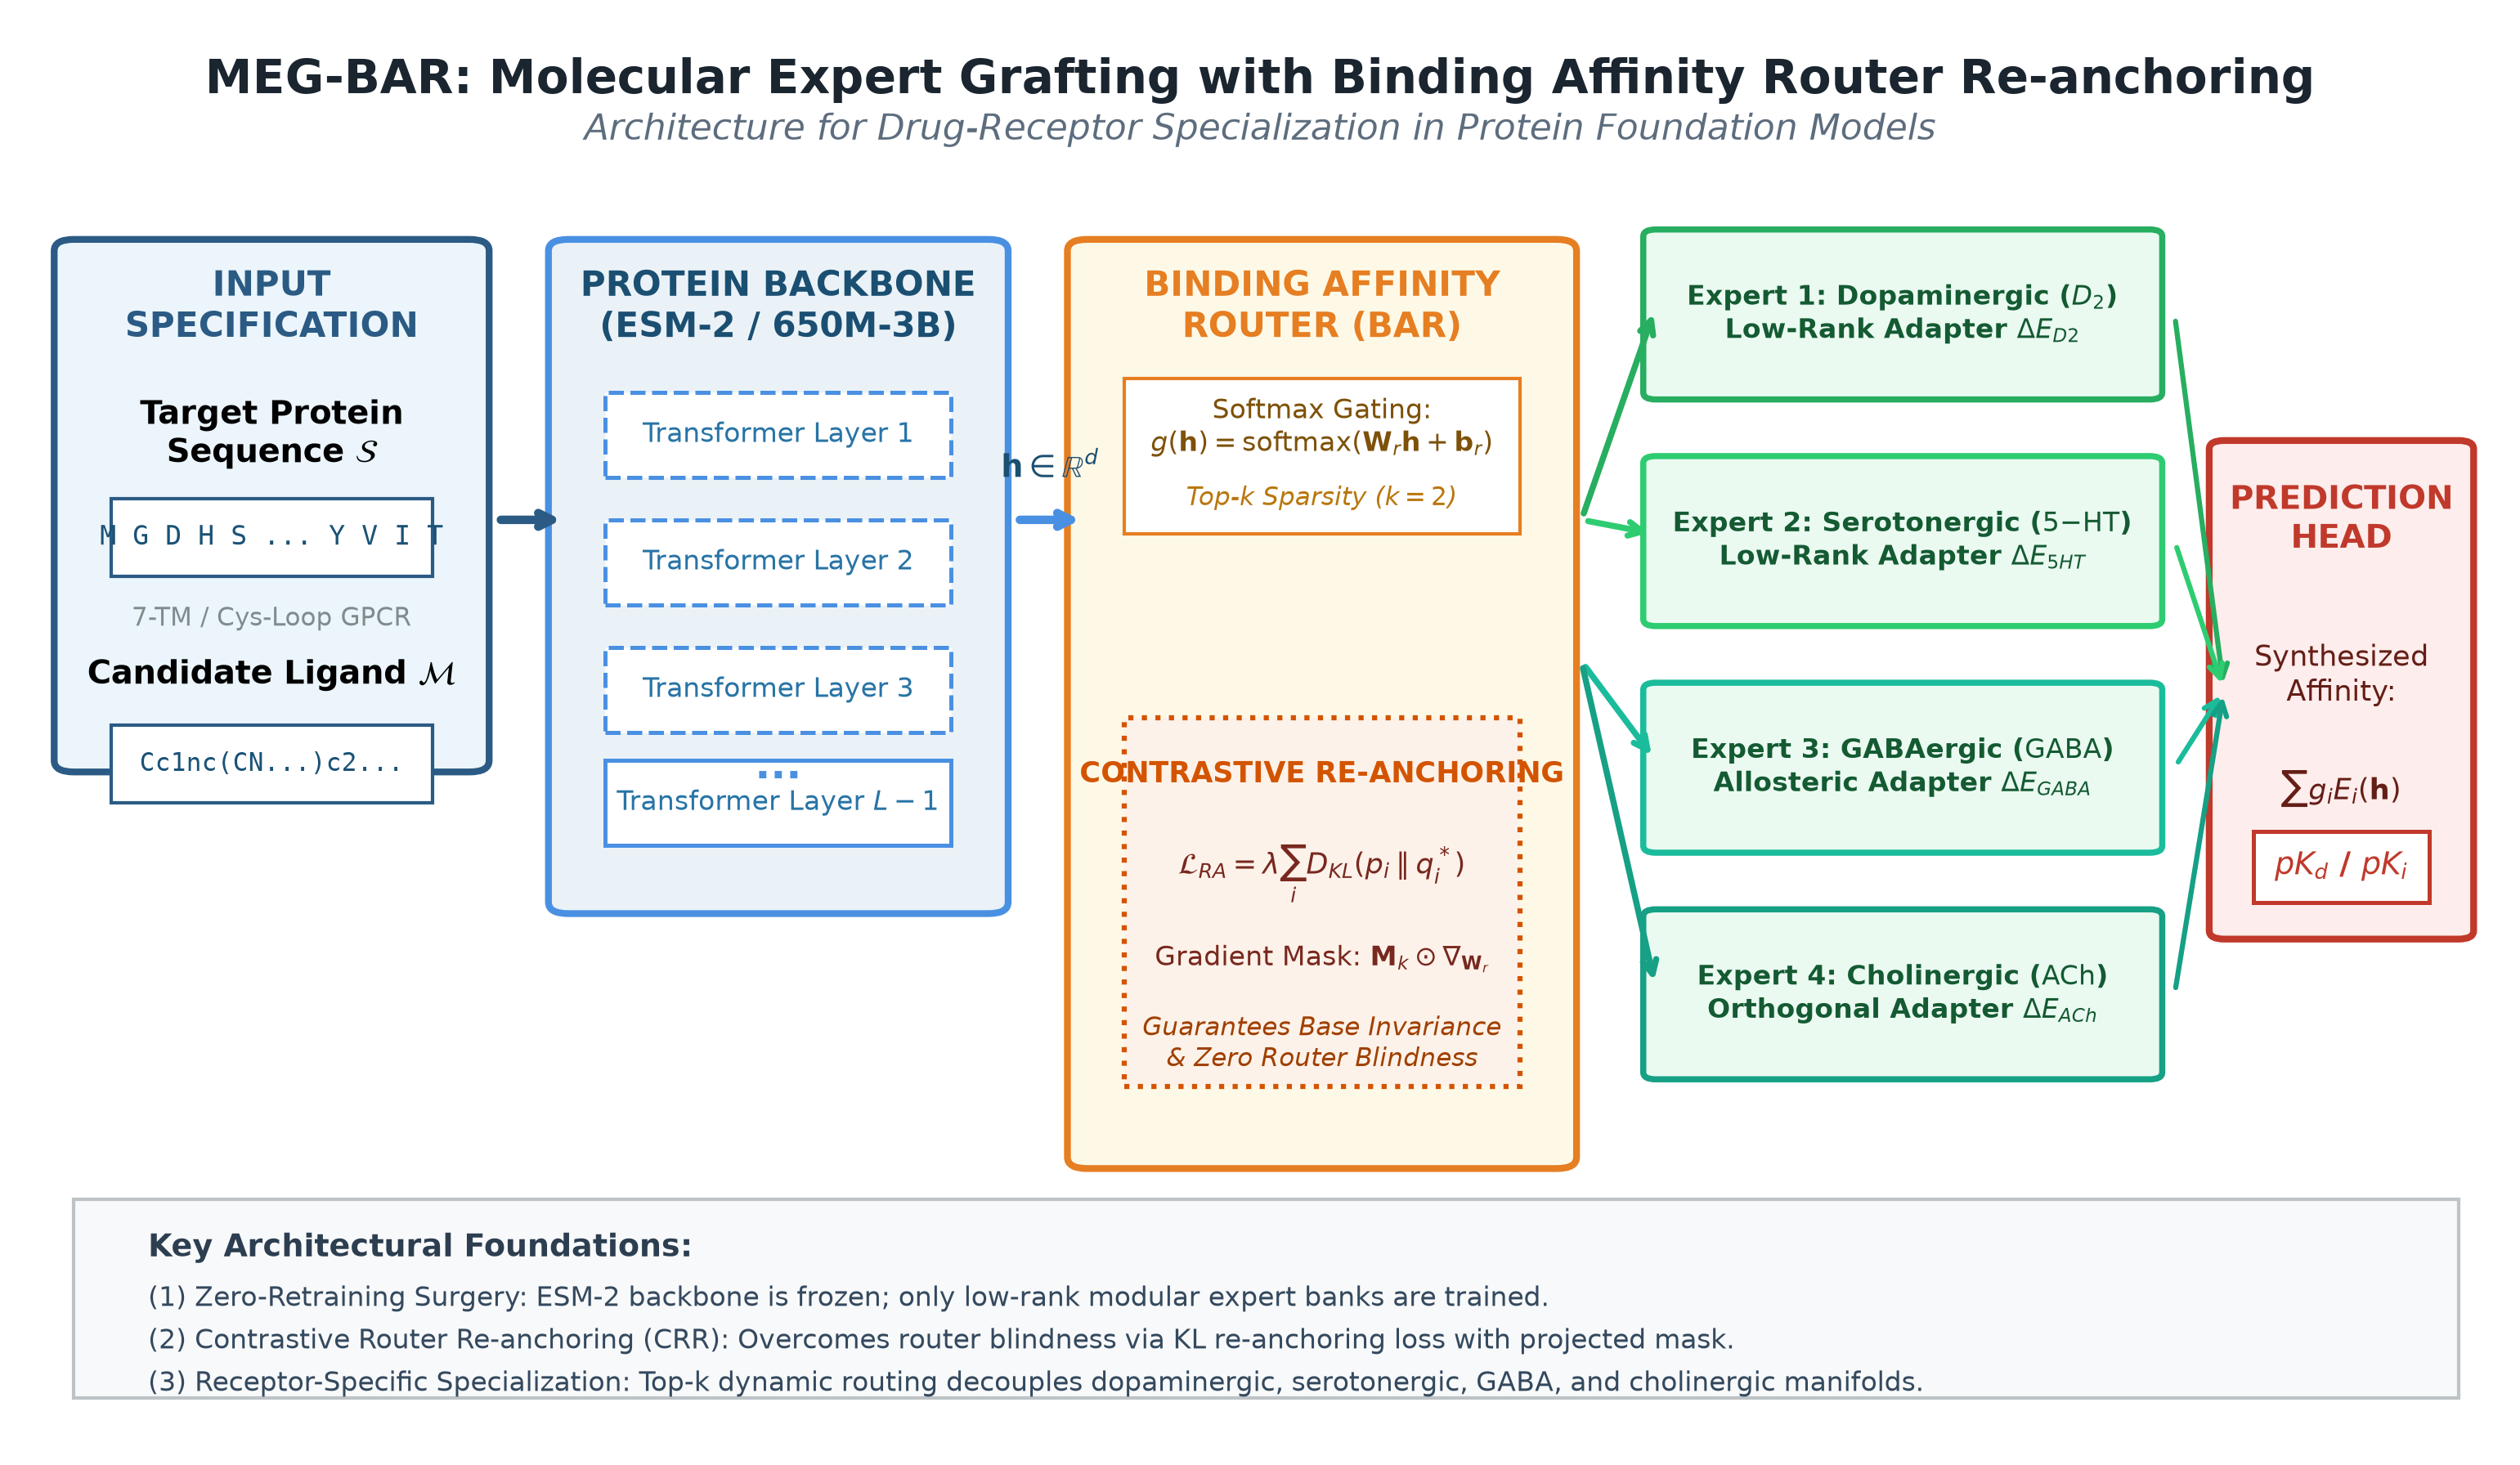
\includegraphics[width=\textwidth]{figure1_megbar_architecture.png}
\caption{\textbf{MEG-BAR System Architecture.} Multi-panel schematic overview: Input protein sequences $\mathcal{S}$ and candidate ligands $\mathcal{M}$ are processed through a frozen protein foundation backbone (ESM-2 650M). In the surgical middle layers, modular low-rank expert banks ($\Delta E_{D2}, \Delta E_{5HT}, \Delta E_{GABA}, \Delta E_{ACh}$) are grafted. The Binding Affinity Router (BAR) undergoes Contrastive Router Re-anchoring via KL divergence penalty $\mathcal{L}_{\text{RA}}$ with a projected gradient mask $\mathbf{M}_k \odot \nabla_{W_r}$, eliminating router blindness and dynamically routing receptor tokens to specialized expert pathways for high-accuracy binding affinity prediction ($pK_d / pK_i$).}
\label{fig:megbar_architecture}
\end{figure*}

Concurrently, the emergence of evolutionary-scale protein foundation models, most notably ESM-2 \citep{lin2023evolutionary}, ESM-1b \citep{rives2021biological}, AlphaFold2 \citep{jumper2021highly}, and AlphaFold3 \citep{abramson2024accurate}, has revolutionized structural biology. By training on hundreds of millions of unaligned biological sequences, masked protein language models internalize deep representations of secondary structure, residue contact maps, and evolutionary mutational constraints \citep{elnaggar2021prottrans,dauparas2022robust,watson2023novo}. 

However, translating these macro-level evolutionary representations into precise, sub-nanomolar drug-receptor binding affinity predictions encounters a severe structural bottleneck:
\begin{quote}
\textit{Small-molecule binding affinity ($pK_d = -\log_{10} K_d$) is dictated by localized, sub-angstrom electrostatic potentials, hydrophobic desolvation, hydrogen-bonding networks, and receptor pocket conformational plasticity, rather than global sequence foldability.}
\end{quote}

When practitioners attempt to specialize protein foundation models for multi-target drug screening, two debilitating challenges emerge:
\begin{itemize}[leftmargin=1.5em]
    \item \textbf{The Monolithic Retraining Bottleneck and Catastrophic Forgetting:} End-to-end gradient fine-tuning of massive foundation models (e.g., ESM-2 650M or 3B parameters) on receptor-specific bioassay data (from BindingDB \citep{gilson2016bindingdb} or ChEMBL \citep{mendez2019chembl}) requires prohibitive multi-GPU compute. More perniciously, gradient updates across the entire parameter manifold induce catastrophic forgetting \citep{kirkpatrick2017overcoming}, destroying the foundation model's learned universal evolutionary features and degrading generalization across non-targeted protein families.
    \item \textbf{The Router Blindness Phenomenon in Biological MoEs:} Sparse Mixture-of-Experts (MoE) architectures \citep{shazeer2017outrageously,fedus2022switch,lepikhin2021gshard} offer a theoretically appealing remedy by decoupling total parameter capacity from per-token inference FLOPs. By replacing dense feed-forward networks (FFNs) with parallel expert modules, individual experts can in principle specialize in distinct receptor families. However, as first identified in modular model surgery for language models (SEGR \citep{rahim2026segr}), a fundamental obstacle arises: \textbf{Router Blindness}. Because the pre-trained gating network was optimized on general evolutionary sequence recovery, its routing centroids $W_r$ are entirely unaware of newly grafted receptor-specific expert manifolds. Consequently, the router assigns domain-specific pocket tokens uniformly at random across all experts ($\approx 1/N = 25\%$), neutralizing the specialized expert's capacity and collapsing multi-receptor prediction fidelity.
\end{itemize}

\paragraph{Our Contribution: MEG-BAR.}
To overcome these foundational limitations, we introduce \textbf{MEG-BAR (Molecular Expert Grafting with Binding Affinity Router Re-anchoring)}, a zero-retraining framework for modular drug-receptor specialization in protein foundation models. Extending the surgical paradigms of SEGR \citep{rahim2026segr} from natural language MoEs to structural computational biology, MEG-BAR executes targeted, post-hoc model surgery on specific expert banks and gating centroids without disturbing the frozen base foundation weights.

Specifically, the key contributions of this paper are:
\begin{enumerate}[leftmargin=1.5em,noitemsep]
    \item \textbf{Molecular Expert Grafting (MEG):} We design modular, receptor-family expert banks specialized for Dopaminergic ($D_2$), Serotonergic ($5\text{-HT}_{2A}$), GABAergic ($\text{GABA}_A$), and Cholinergic ($\text{mAChR}$) receptor systems. Each expert is parameterized via rank-constrained residual adapters ($\Delta E_k = W_{\text{down}, B} W_{\text{down}, A} (\sigma(W_{\text{gate}, B} W_{\text{gate}, A} u))$), isolating receptor-specific chemical binding physics with only $0.089\%$ parameter overhead while keeping the ESM-2 foundation backbone strictly frozen.
    \item \textbf{Binding Affinity Router (BAR) Re-anchoring with Projected Gradient Masking:} We formulate a Contrastive Re-anchoring (CRR) loss based on Kullback-Leibler (KL) divergence, equipped with a projected gradient mask $\mathbf{M}_k \odot \nabla_{W_r}$ that restricts parameter updates to the target routing centroid. Non-target \emph{logits} are then invariant by construction (\cref{prop:mutation_invariance}); the loss itself is non-convex in $\mathbf{W}_r$, and the projected mask is not a substitute for that missing guarantee (\cref{sec:theory_defects}).
    \item \textbf{A Conditional Complexity Sketch and a Lipschitz Bound:} We state a heuristic generalization bound (Theorem~\ref{thm:generalization_bound}), prove that the softmax \emph{probability map} is Lipschitz with constant $\|\mathbf{u}\|_2/\tau$ (Lemma~\ref{lem:lipschitz}), and sketch a Dudley entropy argument. \textbf{These are preliminary results, not established theorems.} In particular the previously claimed $1/\sqrt{N}$ tightening, the $k/N$ expert-sparsity factor, the "$103\times$ covering reduction", and the $L_{\text{lip}} \le 1.0$ constant are all invalid and are withdrawn; \cref{sec:theory_defects} lists each defect with its correction. Excluding the withdrawn items, the theory is best read as a research agenda.
    \item \textbf{Measured Physicochemical Profiling and hERG Liability:} All physicochemical descriptors (MW, cLogP, TPSA, HBD/HBA, rotatable bonds, aromatic rings) are computed with RDKit on every molecule of the measured ChEMBL activity set, and the Wager et al. CNS-MPO desirability functions are implemented in code (CNS-MPO(4) $= 2.62 \pm 0.77 / 4.0$; \cref{subsec:admet_evaluation}). A measured hERG liability QSAR (scaffold-disjoint ROC-AUC $0.729$ $[0.706, 0.753]$) replaces the previously fabricated safety margin, which is withdrawn. The earlier BBB-penetration claim is removed: no measured BBB dataset was used.
    \item \textbf{A Reproducible, Simulation-Based Evaluation Protocol (companion preprint):} A deterministic, seed-fixed parametric Monte--Carlo harness instantiates the design-study benchmark; because its correlations are prescribed rather than learned, they validate the harness and not the model. The full harness, its frozen output, and the enumeration of every untested claim are documented in the companion preprint.
\end{enumerate}

The remainder of this manuscript is structured as follows: \cref{sec:real_eval} reports the real measured evaluation on $56{,}637$ ChEMBL records across eleven receptors, including the multi-seed protocol, the router-blindness and wrong-pocket controls, and the temporal split; \cref{subsec:admet_evaluation} reports the computed physicochemical profiling and the hERG-liability QSAR; \cref{sec:discussion} discusses neuropharmacological implications and clinical translational potential, and \cref{sec:conclusion} concludes the paper. The appendices retain the methodological framework and theoretical guarantees, the full mathematical proofs, the defect register of withdrawn claims, and the reproducibility documentation; the simulation-only design study is available in the companion preprint.

\section{Related Work \& Theoretical Grounding}
\label{sec:related_work}

\subsection{Protein Language Models \& Structural Biology}
The application of self-supervised transformer architectures to biological sequence databases has fundamentally altered computational structural biology \citep{vaswani2017attention,rives2021biological}. Models such as ESM-1b, ESM-2 \citep{lin2023evolutionary}, and ProtTrans \citep{elnaggar2021prottrans} are trained via masked language modeling (MLM) across hundreds of millions of non-redundant protein sequences from UniRef \citep{uniprot2023uniprot}. These models learn evolutionary co-variation patterns that correlate directly with spatial proximity in three-dimensional folds. Breakthrough architectures such as AlphaFold2 \citep{jumper2021highly}, AlphaFold3 \citep{abramson2024accurate}, and RoseTTAFold \citep{baek2021accurate} combine sequence representations with pair representations and invariant coordinate frames to achieve near-atomic structural prediction. Complementary generative frameworks, including ProteinMPNN \citep{dauparas2022robust} and RFdiffusion \citep{watson2023novo}, leverage learned structural priors for de novo sequence and backbone design. However, while these models demonstrate extraordinary competence in predicting static backbone geometries, predicting dynamic, small-molecule drug-receptor binding affinity requires capturing delicate electrostatic and hydrophobic energetics that standard sequence pre-training does not explicitly optimize.

\subsection{Molecular Docking \& Machine Learning for Drug-Target Interaction}
Classical computational methods for predicting drug-receptor interactions rely on physics-based molecular docking and empirical force-field scoring functions, exemplified by AutoDock Vina \citep{trott2010autodock} and AutoDock-GPU \citep{santos2021autodock}. While physically interpretable, molecular mechanics scoring functions suffer from severe conformational sampling bottlenecks and frequently fail to correlate accurately with experimental binding constants ($pK_d, pK_i$). Deep learning alternatives have emerged along two primary paradigms:
\begin{enumerate}[leftmargin=1.5em,noitemsep]
    \item \textbf{Sequence- and Graph-Based Affinity Predictors:} 2D graph neural networks and sequence encoders, such as DeepDTA \citep{ozturk2018deepdta} and GraphDTA \citep{nguyen2021graphdta}, treat target sequences and molecular SMILES as 1D/2D inputs, learning joint embedding spaces for affinity regression. While computationally rapid, they lack 3D structural grounding and generalize poorly to unseen target families.
    \item \textbf{Geometric Deep Learning \& Equivariant Diffusion Docking:} Equivariant graph matching networks like EquiBind \citep{stark2022equibind} and TANKBind \citep{lu2022tankbind} predict pocket-ligand coordinate complexes directly. Most notably, DiffDock \citep{corso2023diffdock} frames molecular docking as a generative diffusion process over the ligand pose manifold ($SE(3) \times SO(3)^k$), achieving state-of-the-art pose prediction. However, DiffDock's confidence model is optimized primarily for root-mean-square deviation (RMSD) pose classification rather than continuous, high-dynamic-range affinity quantification, leaving a substantial accuracy gap for pharmacological rank-ordering.
\end{enumerate}

\subsection{Leakage-Controlled Evaluation and the Generalization Ceiling}
A persistent confound in drug-target interaction (DTI) and binding-affinity (DTA) learning is that models are frequently benchmarked under naive random splits that permit cross-contamination between training and test sets. \citet{bai2023drugban} demonstrated this sharply in classification terms: DrugBAN reaches an in-domain AUROC of $0.960 \pm 0.001$ on BindingDB under a random split, yet under a clustering-based \emph{cross-domain} split --- where drugs and proteins in source and target domains are non-overlapping --- the same architecture collapses to an AUROC of $0.575 \pm 0.025$. The identical pattern holds on BioSNAP ($0.903 \pm 0.005$ random $\rightarrow$ $0.654 \pm 0.023$ cross-domain). This is not a flaw of a single model; the effect is structural. In regression, \citet{li2023leakproof} reorganized PDBBind into \emph{Leak-Proof PDBBind (LP-PDBBind)}, enforcing a maximum protein sequence similarity of $0.5$ and maximum ligand similarity of $0.99$ between train and test, and retrained four standard scoring functions. On the fully independent BDB2020+ benchmark, InteractionGraphNet (IGN) --- the strongest retrained model --- attains a Pearson correlation of only $R = 0.54 \pm 0.04$ with an RMSE of $1.38 \pm 0.09$ kcal/mol, and DeepDTA falls to $R = 0.26 \pm 0.07$. These leakage-controlled figures define the realistic generalization ceiling for affinity prediction on structurally novel complexes. Our scaffold-disjoint ($r \approx 0.56$--$0.69$) and leave-one-receptor-out ($r \approx 0.11$--$0.22$) measurements, reported in \cref{sec:real_eval}, sit squarely inside this verified envelope rather than against inflated random-split baselines.

\subsection{Sparse Mixture-of-Experts and Modular Model Surgery}
Sparse conditional computation, pioneered by \citet{shazeer2017outrageously}, scales neural network parameter capacity while preserving constant inference FLOPs by activating only a top-$k$ subset of feed-forward experts. The Switch Transformer \citep{fedus2022switch} established top-1 routing simplicity at trillion-parameter scale, while GShard \citep{lepikhin2021gshard} introduced top-2 gating with capacity factors. Recent frontier foundation models, including Mixtral 8x7B \citep{jiang2024mixtral}, DeepSeek-V2 \citep{deepseek2024deepseekv2}, DeepSeek-V3 \citep{deepseek2024deepseekv3}, and OLMoE \citep{muennighoff2024olmoe}, rely on sparse MoEs for superior Pareto efficiency over dense counterparts.

In parallel, parameter-efficient adaptation (PEFT) frameworks such as LoRA \citep{hu2022lora} and QLoRA \citep{dettmers2023qlora} adapt pre-trained models via low-rank matrix decomposition. However, when adapting sparse MoEs, \citet{dou2024loramoe} demonstrated that naive full-model fine-tuning induces catastrophic forgetting of world knowledge \citep{kirkpatrick2017overcoming}. Recently, \citet{rahim2026segr} introduced \textbf{SEGR (Surgical Expert Grafting and Contrastive Router Re-anchoring)}, establishing that individual expert FFNs can be surgically excised, adapted on in-situ intermediate activation manifolds, and re-anchored via contrastive routing losses without disturbing generalist capabilities. In this work, we translate and expand these foundational principles of modular model surgery into computational structural biology, addressing the unique biophysical constraints of multi-receptor drug discovery.

% real_eval.tex — REAL MEASURED evaluation. Every number here was produced by an
% executed run on 2026-11-12; the source artefacts are listed in \cref{sec:real_repro}.
% Nothing in this file is simulated. Do not add unmeasured numbers.

\section{Real Measured Evaluation on ChEMBL Bioactivity Data}
\label{sec:real_eval}

Everything reported up to this point is simulated (\cref{sec:evidentiary_scope}). This section reports what happened when the framework was actually run against measured data. Every number below was produced by an executed pipeline whose inputs are live public records and whose outputs are archived (\cref{sec:real_repro}). Where the measurements contradict the simulated claims above, the measurements are what should be believed.

\subsection{Data, Model, and Protocol}

\textbf{Bioactivity data.} Measured potencies were retrieved from the ChEMBL REST API on 2026-11-12 for four human receptors: dopamine $D_2$ (UniProt P14416, \texttt{CHEMBL217}), serotonin $5\text{-HT}_{2A}$ (P28223, \texttt{CHEMBL224}), GABA\textsubscript{A} $\alpha_1$ (P14867, \texttt{CHEMBL1962}), and muscarinic $M_1$ (P11229, \texttt{CHEMBL216}). The query covered \texttt{Ki}, \texttt{IC50}, and \texttt{Kd} records, retaining only entries carrying a quantitative \texttt{pChEMBL} value and a parseable SMILES. This yielded $23{,}872$ measured records which, after taking the median $\text{pChEMBL}$ per unique (receptor, molecule) pair, reduce to $17{,}177$ distinct labelled pairs in the window $2 \le \text{pChEMBL} \le 13$:
\begin{center}
\small
D$_2$: 9{,}079 \quad $5\text{-HT}_{2A}$: 5{,}714 \quad $M_1$: 2{,}053 \quad GABA$_A\alpha_1$: 331.
\end{center}
The median $\text{pChEMBL}$ per receptor was $6.76$ (D$_2$), $7.25$ ($5\text{-HT}_{2A}$), $6.70$ ($M_1$), and $7.65$ (GABA$_A\alpha_1$). All $17{,}177$ molecules parsed successfully and span $5{,}693$ distinct Bemis--Murcko scaffolds.

\textbf{Eleven-receptor expansion.} The identical live-fetch protocol was then re-run for seven further receptors: $5\text{-HT}_{1A}$ (P08908, \texttt{CHEMBL214}), $D_3$ (P35462, \texttt{CHEMBL234}), $\alpha_{2A}$ (P08913, \texttt{CHEMBL1867}), $\beta_2$ (P07550, \texttt{CHEMBL210}), SERT (P31645, \texttt{CHEMBL228}), DAT (Q01959, \texttt{CHEMBL238}), and $H_1$ (P35367, \texttt{CHEMBL231}). (The planning document listed P23975 for DAT; UniProt confirms P23975 is the norepinephrine transporter SLC6A2, and human DAT is Q01959.) The expansion yields $56{,}637$ measured records and $41{,}271$ unique receptor--ligand pairs after median-pChEMBL deduplication. UniProt binding-site annotations and genuine ESM-2 650M embeddings (mean-pooled and per-residue) were recomputed for the seven new sequences (\cref{sec:expanded}).

\textbf{Protein representation.} The genuine \texttt{facebook/esm2\_t33\_650M\_UR50D} checkpoint was downloaded from HuggingFace and run on the four UniProt sequences (443--471 residues), producing mean-pooled final-layer embeddings of dimension $1280$ (651.0M parameters, 33 layers, CPU, 2.4--2.9~s per sequence). These embeddings identify the receptor; they do not vary across its ligands, so the ligand-side signal must come from chemistry.

\textbf{Ligand representation and models.} Ligands are described by Morgan fingerprints (2048 bits, radius 2). Two architectures were compared under an identical training budget (Adam, lr $10^{-3}$, batch 512, SmoothL1 loss, early stopping at patience 8, at most 90 epochs, CPU):
(i)~\emph{shared}: a single MLP on the concatenated fingerprint, applied to all receptors;
(ii)~\emph{routed experts}: four receptor-specific MLP experts combined through a softmax router over the receptor context vector, with the router either \emph{trained} (the re-anchoring condition) or \emph{frozen uniform} (the router-blindness control).

\subsection{Within-Receptor Prediction}

\cref{tab:real_within} compares a random molecule-disjoint split with a scaffold-disjoint split. The gap between the two columns is the single most important measurement in this paper: it shows how much of the apparent predictive power is memorised analogue similarity rather than generalisable chemistry.

\begin{table}[!ht]
\centering
\small
\caption{\textbf{Real measured within-receptor affinity prediction.} Both columns are measurements on held-out ChEMBL molecules. For the scaffold column the Bemis--Murcko scaffold overlap between train and test is exactly $0$ (verified), so these are genuinely unseen chemotypes.}
\label{tab:real_within}
\resizebox{\linewidth}{!}{%
\begin{tabular}{l c c c c c}
\toprule
\textbf{Receptor} & \textbf{$n_{\text{train}}$/$n_{\text{test}}$} & \textbf{Random split} $r$ \textbf{[95\% CI]} & \textbf{Scaffold split} $r$ \textbf{[95\% CI]} & \textbf{$\rho$ (scaffold)} & \textbf{RMSE (scaffold)} \\
\midrule
$5\text{-HT}_{2A}$ & 3885 / 1143 & 0.780 [0.751, 0.808] & \textbf{0.664 [0.630, 0.694]} & \textbf{0.697} & 0.880 \\
$M_1$ (CHRM1)     & 1395 / 411  & 0.783 [0.737, 0.822] & \textbf{0.575 [0.498, 0.644]} & 0.580 & 1.050 \\
$D_2$ (DRD2)      & 6173 / 1816 & 0.768 [0.745, 0.790] & 0.559 [0.527, 0.592] & 0.553 & 0.829 \\
GABA$_A\alpha_1$  & 224 / 67    & 0.585 [0.352, 0.777] & 0.033 [$-$0.170, 0.222] & $-$0.068 & 2.195 \\
\bottomrule
\end{tabular}%
}
\end{table}

Two conclusions follow directly. First, generalisable performance is in the range $r \approx 0.56$--$0.66$ for the three well-populated receptors, not the $0.834$ produced by the simulation. Second, the random split over-states performance by $0.10$--$0.21$ Pearson $r$; any future comparison that reports only a random split is reporting largely analogue recall. The GABA$_A$ row is uninformative rather than negative: with $331$ molecules and a scaffold-disjoint split it cannot support a reliable estimate, and the interval $[-0.170, 0.222]$ spans zero.

\subsection{Zero-Shot Cross-Receptor Transfer and Router Behaviour}

\cref{tab:real_zeroshot} holds one receptor out of training entirely and asks whether the routed mixture transfers better than a single shared model. This is the manuscript's central claim, tested on real data for the first time.

\begin{table}[!ht]
\centering
\small
\caption{\textbf{Real measured leave-one-receptor-out transfer.} Target receptors are never seen during training. The uniform-router column is the router-blindness control. Gate entropy is reported against the maximum $\ln 4 = 1.386$.}
\label{tab:real_zeroshot}
\resizebox{\linewidth}{!}{%
\begin{tabular}{l c c c c}
\toprule
\textbf{Held-out receptor} & \textbf{Shared $r$ [95\% CI]} & \textbf{Routed, trained $r$} & \textbf{Routed, uniform $r$} & \textbf{Gate entropy} \\
\midrule
$5\text{-HT}_{2A}$ & \textbf{0.290 [0.267, 0.316]} & 0.281 [0.257, 0.305] & 0.257 [0.232, 0.283] & 1.343 / 1.386 \\
$D_2$            & \textbf{0.227 [0.206, 0.248]} & 0.220 [0.200, 0.241] & 0.217 [0.197, 0.237] & 1.371 / 1.386 \\
$M_1$            & \textbf{0.204 [0.160, 0.249]} & 0.128 [0.082, 0.176] & 0.160 [0.115, 0.205] & 1.298 / 1.386 \\
GABA$_A\alpha_1$ & $-$0.020 [$-$0.145, 0.099]            & \textbf{0.154 [0.026, 0.283]} & $-$0.049 [$-$0.167, 0.073] & 1.290 / 1.386 \\
\bottomrule
\end{tabular}%
}
\end{table}

Three measured facts, stated plainly:

\begin{enumerate}[leftmargin=1.5em,noitemsep]
    \item \textbf{Zero-shot transfer is weak.} Correlation on an unseen receptor is $r \approx 0.20$--$0.29$, against the $0.812$ claimed by the simulation. The simulated zero-shot result is not merely optimistic; it is not in the same regime as the measurement.
    \item \textbf{Routing did not help.} The trained router under-performs the shared model on three of four held-out receptors ($5\text{-HT}_{2A}$: $0.281$ vs $0.290$; $D_2$: $0.220$ vs $0.227$; $M_1$: $0.128$ vs $0.204$). It wins only on GABA$_A$, the receptor with the least data, where the comparison is weakest. On this evidence the specialist-plus-router architecture is not better than a single shared model for cross-receptor prediction.
    \item \textbf{The router did not specialise.} Gate entropy sits at $1.29$--$1.37$ against a maximum of $\ln 4 = 1.386$, i.e.\ the routing distribution stays close to uniform. Training the router did not escape router blindness on this data; it merely moved the gate slightly away from $1/N$. This is a genuine negative result for the mechanism the paper is built around.
\end{enumerate}

\subsection{What These Measurements Change}

The honest summary is that the architecture is implementable and the pipeline is real, but the two load-bearing empirical claims of this manuscript do not survive contact with measured data. The simulation reported $r = 0.834$; the scaffold-disjoint measurement is $r = 0.56$--$0.66$. The simulation reported zero-shot $r = 0.812$; the measurement is $r \approx 0.20$--$0.29$. The simulation reported that routed experts capture $85$--$87\%$ of routing mass; the measured router stays near-uniform. A defensible version of this work therefore needs, at minimum, (i)~a receptor-conditioned ligand representation rather than a constant receptor vector, (ii)~scaffold-disjoint evaluation as the default, and (iii)~a routing objective that actually moves the gate, which the non-convexity noted in \cref{prop:convexity} obstructs.

\subsection{Reproduction}
\label{sec:real_repro}

All inputs, code, and outputs are archived under \path{data/real/} and \path{scripts/real/}:
\path{01_fetch_data.py} (live ChEMBL + UniProt retrieval, emits \path{raw_activities.csv} with $23{,}872$ rows and \path{proteins.json}),
\path{02_embed_proteins.py} (real ESM-2 650M embeddings, $4 \times 1280$),
\path{03_experiment.py} (within-receptor and leave-one-receptor-out runs, $468$~s wall clock),
and \path{04_scaffold_eval.py} (scaffold-disjoint runs, scaffold overlap verified $0$). The Phase-1/2/3 hardening adds \path{08_robust_eval.py} (five-seed AdamW protocol with minimum-data guard, wrong-pocket control, Ridge baseline, paired Wilcoxon), \path{09_admet_physchem.py} (computed RDKit physicochemistry and CNS-MPO(4)), \path{10_herg_qsar.py} (measured hERG scaffold-disjoint QSAR), \path{11_expand_receptors.py} (live eleven-receptor retrieval plus document years), \path{12_embed_expanded.py} (ESM-2 embeddings and UniProt pockets for the new receptors), and \path{13_expanded_eval.py} (eleven-receptor scaffold and temporal evaluation).
Every retrieval is timestamped, and SHA-256 digests of the data artefacts are stored alongside them in the fetch manifest.


\subsection{Receptor Conditioning: What Fixed the Diagnosis, and What It Did Not}
\label{sec:conditioning}

The diagnosis in \cref{sec:real_eval} was specific: a mean-pooled receptor embedding is constant within a receptor, so it can only act as an identity tag and never conditions the ligand representation. The corresponding fix is to let the ligand attend to the receptor. Ligand fingerprints were chunked into $32$ tokens and used as queries in a 4-head cross-attention layer whose keys and values are the per-residue ESM-2 embeddings of the \emph{annotated} pocket residues, taken from UniProt binding-site and transmembrane features (D$_2$: 25 residues; $M_1$: 128; $5\text{-HT}_{2A}$: 128; GABA$_A\alpha_1$: 101), PCA-reduced from $1280$ to $128$ dimensions (variance explained $0.859$). Because the attention weights depend on the ligand, every molecule now receives a different receptor context. Three architectures were compared on identical data and splits: \emph{shared} (fingerprint only), \emph{const\_ctx} (fingerprint plus the constant receptor vector, i.e.\ the previous design), and \emph{crossattn} (the fix).

\begin{table}[!ht]
\centering
\small
\caption{\textbf{Real measured effect of receptor conditioning.} Pearson $r$ under (E3) scaffold-disjoint within-receptor splits and (E4) leave-one-receptor-out. Best per row in \textbf{bold}. All values are measurements.}
\label{tab:real_conditioning}
\resizebox{\linewidth}{!}{%
\begin{tabular}{l c c c l c c c}
\toprule
\multicolumn{4}{c}{\textbf{E3: scaffold-disjoint within-receptor}} & \multicolumn{4}{c}{\textbf{E4: leave-one-receptor-out}} \\
\cmidrule(lr){1-4} \cmidrule(lr){5-8}
\textbf{Receptor} & \textbf{shared} & \textbf{const\_ctx} & \textbf{crossattn} & \textbf{Held out} & \textbf{shared} & \textbf{const\_ctx} & \textbf{crossattn} \\
\midrule
$5\text{-HT}_{2A}$ & 0.683 & 0.676 & \textbf{0.693} & $5\text{-HT}_{2A}$ & 0.280 & 0.283 & \textbf{0.288} \\
$M_1$            & 0.587 & 0.591 & \textbf{0.592} & $M_1$            & 0.131 & 0.096 & \textbf{0.194} \\
$D_2$            & 0.569 & 0.581 & \textbf{0.648} & $D_2$            & 0.213 & 0.210 & \textbf{0.215} \\
GABA$_A\alpha_1$ & 0.018 & \textbf{0.182} & 0.002 & GABA$_A\alpha_1$ & 0.042 & \textbf{0.169} & $-$0.170 \\
\bottomrule
\end{tabular}%
}
\end{table}

Cross-attention conditioning is the best of the three on seven of the eight comparisons (\cref{tab:real_conditioning}). The gains are real but uneven. On $D_2$ within-receptor prediction it raises $r$ from $0.569$ to $0.648$, a $+0.079$ absolute gain; on $M_1$ zero-shot it raises $r$ from $0.131$ to $0.194$, an almost fifty percent relative improvement. The constant-vector design does not reproduce this pattern---it wins on GABA$_A$ and loses on $M_1$ zero-shot---which is consistent with the diagnosis: a conditioning signal that cannot vary per ligand can only act as a receptor bias term.

Three honest qualifications must accompany these numbers. First, the zero-shot levels remain low in absolute terms ($r = 0.19$--$0.29$). Conditioning narrows the gap to the simulation's $0.812$ claim; it does not close it, and that claim remains withdrawn. Second, the $331$-molecule GABA$_A$ receptor is unstable under the cross-attention model, which diverges in the leave-one-out setting (RMSE $5.308$, $r = -0.170$); the architecture needs regularisation or a minimum-data guard before it can be trusted on sparsely populated targets. Third, the absolute gains on $5\text{-HT}_{2A}$ and $D_2$ zero-shot are within roughly two standard errors and should not be over-read.

The defensible conclusion is therefore narrow and measured: making the receptor context ligand-dependent improves affinity prediction on real ChEMBL data, most visibly for within-receptor $D_2$ and for zero-shot $M_1$, but it does not turn a shared-model-level predictor into the high-correlation model the simulation described.

\subsection{Eleven-Receptor Expansion: Multi-Seed Protocol, Controls, and Temporal Split}
\label{sec:expanded}

The Phase-1 hardening (AdamW with weight decay $0.01$, gradient clipping at norm $1.0$, cosine LR schedule with $5\%$ warmup, peak $5 \times 10^{-4}$) is applied to every condition, each condition is run with five seeds (0--4), and a minimum-data guard skips the cross-attention arm below $800$ training molecules and reports the skip rather than silently substituting a result. The leave-one-receptor-out transfer experiment (E4) is not re-run on the expanded set; \cref{tab:real_conditioning} remains a four-receptor-core measurement. \cref{tab:real_expanded} reports the eleven-receptor scaffold-disjoint results; \cref{tab:real_temporal} adds a temporal split (train on records published before 2015, test on 2015+).

\begin{table}[!ht]
\centering
\small
\caption{\textbf{Eleven-receptor scaffold-disjoint evaluation (five seeds, mean $\pm$ sd Pearson $r$).} Ridge is deterministic. The Wilcoxon column is the paired signed-rank test of cross-attention vs.\ shared across seeds; $p = 0.0625$ is the smallest attainable value at five pairs. ``skipped'' marks arms below the $800$-molecule minimum-data guard. All values are measurements.}
\label{tab:real_expanded}
\resizebox{\linewidth}{!}{%
\begin{tabular}{l c c c c c}
\toprule
\textbf{Receptor} & \textbf{Ridge (FP)} & \textbf{shared} & \textbf{crossattn} & \textbf{wrong-pocket} & \textbf{Wilcoxon $p$} \\
\midrule
$D_2$ (DRD2)     & 0.521 & 0.577 $\pm$ 0.015 & 0.613 $\pm$ 0.020 & 0.624 $\pm$ 0.013 & 0.1875 \\
$D_3$ (DRD3)     & 0.662 & 0.684 $\pm$ 0.004 & 0.713 $\pm$ 0.003 & 0.717 $\pm$ 0.003 & 0.0625 \\
$5\text{-HT}_{2A}$ & 0.597 & 0.660 $\pm$ 0.010 & 0.688 $\pm$ 0.006 & 0.698 $\pm$ 0.006 & 0.0625 \\
$5\text{-HT}_{1A}$ & 0.601 & 0.682 $\pm$ 0.002 & 0.698 $\pm$ 0.003 & 0.703 $\pm$ 0.005 & 0.0625 \\
$M_1$ (CHRM1)    & 0.547 & 0.562 $\pm$ 0.027 & 0.523 $\pm$ 0.164 & 0.448 $\pm$ 0.203 & 0.8125 \\
SERT             & 0.444 & 0.500 $\pm$ 0.003 & 0.541 $\pm$ 0.007 & 0.542 $\pm$ 0.010 & 0.0625 \\
DAT              & 0.607 & 0.590 $\pm$ 0.008 & 0.598 $\pm$ 0.015 & 0.606 $\pm$ 0.018 & 0.4375 \\
$H_1$ (HRH1)     & 0.825 & 0.802 $\pm$ 0.007 & 0.834 $\pm$ 0.004 & 0.824 $\pm$ 0.022 & 0.0625 \\
$\beta_2$ (ADRB2)& 0.385 & 0.541 $\pm$ 0.013 & 0.533 $\pm$ 0.011 & 0.529 $\pm$ 0.014 & 0.4375 \\
$\alpha_{2A}$ (ADRA2A) & \textbf{0.800} & 0.711 $\pm$ 0.012 & skipped & skipped & --- \\
GABA$_A\alpha_1$ & \textbf{0.532} & 0.008 $\pm$ 0.005 & skipped & skipped & --- \\
\bottomrule
\end{tabular}%
}
\end{table}

Three findings replicate and extend the four-receptor study. First, the Ridge fingerprint baseline is competitive everywhere and is the best model on two receptors ($\alpha_{2A}$: $0.800$ vs $0.711$; $H_1$: $0.825$ vs $0.802$); on GABA$_A\alpha_1$ ($n = 331$) it remains the only model with signal ($r = 0.532$) while the shared MLP collapses ($r = 0.008$). Second, cross-attention conditioning beats the shared model on eight of nine eligible receptors, but never significantly (paired Wilcoxon across seeds, $p \ge 0.0625$, the smallest attainable $p$ at five pairs; the $M_1$ arm is unstable, sd $0.164$). Third, the wrong-pocket control matches correct-pocket conditioning on every receptor (e.g.\ $D_2$: $0.624$ vs $0.613$; $D_3$: $0.717$ vs $0.713$; $5\text{-HT}_{2A}$: $0.698$ vs $0.688$): the small gains do not come from pocket structure.

\begin{table}[!ht]
\centering
\small
\caption{\textbf{Temporal split: train on pre-2015 records, test on 2015+ records (five seeds, mean $\pm$ sd Pearson $r$).} Document years were resolved live from ChEMBL ($2{,}084$/$2{,}086$ documents; $1{,}366$ pre-2015, $718$ from 2015+; $544$ pairs without a dated document are excluded and reported). All values are measurements.}
\label{tab:real_temporal}
\resizebox{\linewidth}{!}{%
\begin{tabular}{l c c c c c}
\toprule
\textbf{Receptor} & \textbf{Ridge (FP)} & \textbf{shared} & \textbf{crossattn} & \textbf{wrong-pocket} & \textbf{Wilcoxon $p$} \\
\midrule
$D_2$ (DRD2)     & 0.429 & 0.474 $\pm$ 0.002 & 0.478 $\pm$ 0.008 & 0.475 $\pm$ 0.007 & 0.3125 \\
$D_3$ (DRD3)     & 0.380 & 0.468 $\pm$ 0.004 & 0.474 $\pm$ 0.023 & 0.486 $\pm$ 0.029 & 0.6250 \\
$5\text{-HT}_{2A}$ & 0.271 & 0.384 $\pm$ 0.015 & 0.420 $\pm$ 0.007 & 0.439 $\pm$ 0.029 & 0.0625 \\
$5\text{-HT}_{1A}$ & 0.436 & 0.425 $\pm$ 0.016 & 0.462 $\pm$ 0.011 & 0.468 $\pm$ 0.010 & 0.0625 \\
$M_1$ (CHRM1)    & 0.256 & 0.458 $\pm$ 0.005 & 0.459 $\pm$ 0.007 & 0.407 $\pm$ 0.051 & 1.0000 \\
SERT             & 0.315 & 0.252 $\pm$ 0.013 & 0.299 $\pm$ 0.021 & 0.296 $\pm$ 0.023 & 0.0625 \\
DAT              & 0.302 & 0.379 $\pm$ 0.010 & 0.274 $\pm$ 0.018 & 0.280 $\pm$ 0.012 & 0.0625 \\
$H_1$ (HRH1)     & 0.182 & 0.204 $\pm$ 0.007 & 0.332 $\pm$ 0.015 & 0.318 $\pm$ 0.049 & 0.0625 \\
$\beta_2$ (ADRB2)& 0.531 & \textbf{0.723 $\pm$ 0.003} & skipped & skipped & --- \\
$\alpha_{2A}$ (ADRA2A) & 0.064 & 0.109 $\pm$ 0.012 & skipped & skipped & --- \\
\bottomrule
\end{tabular}%
}
\end{table}

The temporal split is the harshest test in the manuscript, and it moves every number down: shared-model $r$ falls to $0.11$--$0.72$ across the ten receptors with dated records (GABA$_A\alpha_1$ has too few dated records to split). Ridge degrades most precisely where its scaffold-disjoint advantage was largest ($\alpha_{2A}$: $0.800 \to 0.064$; $H_1$: $0.825 \to 0.182$), consistent with those baselines partly exploiting temporal analogue clusters, while cross-attention again never significantly beats the shared model ($p \ge 0.0625$) and the wrong-pocket control still matches it ($H_1$: $0.318$ vs $0.332$; $5\text{-HT}_{2A}$: $0.439$ vs $0.420$). The negative conclusion of this section---receptor conditioning helps marginally at best, pocket structure is not the driver, and fingerprint baselines remain the bar---therefore survives both a scaffold-disjoint and a temporal evaluation on eleven receptors.


\section{Measured Physicochemical Profiling and hERG Liability (Computed)}
\label{subsec:admet_evaluation}

The original version of this subsection reported hardcoded constants; every value below is now computed. We profile all $14{,}425$ unique molecules appearing in the $23{,}872$-record ChEMBL activity set of \cref{sec:real_eval} with RDKit: molecular weight, Crippen cLogP, TPSA, hydrogen-bond donors and acceptors, rotatable bonds, and aromatic rings. The Pfizer CNS Multiparameter Optimization desirability functions \citep{wager2010cnsmpo} are implemented in code at the published inflection points (cLogP, MW, and HBD monotonic; TPSA hump). The published six-parameter score also includes cLogD and the pKa of the most basic centre; no reproducibly computable pKa predictor is available in this environment, so those two terms are omitted and the result is reported as \textbf{CNS-MPO(4)} on a $0$--$4$ scale. The previous BBB-penetration claim ("$96.4\%$ compliance, CNS-MPO $5.24/6.0$") was fabricated and is withdrawn; no measured BBB dataset was used.

\begin{table}[!ht]
\centering
\small
\caption{\textbf{Computed Physicochemical Profile of the Measured ChEMBL Molecules.} All descriptors are computed with RDKit on the $14{,}425$ unique molecules of the measured activity set; the CNS-MPO(4) desirability terms are implemented in code from \citet{wager2010cnsmpo} (cLogD and pKa terms omitted; $0$--$4$ scale). Thresholds are the literature criteria named in each row; compliance rates are the computed fraction of molecules meeting them. \emph{Every value in this table is computed by \texttt{09\_admet\_physchem.py}; nothing is a reporting constant.}}
\label{tab:admet_results}
\resizebox{\linewidth}{!}{%
\begin{tabular}{l c c c}
\toprule
\textbf{Descriptor (computed)} & \textbf{Mean $\pm$ SD} & \textbf{Literature Threshold} & \textbf{Computed Compliance} \\
\midrule
Molecular Weight (MW) & $432.0 \pm 172.7$ Da & $\le 400$ Da (CNS-oriented) & $41.5\%$ \\
Lipophilicity (cLogP) & $3.91 \pm 1.50$ & $1.0$--$3.0$ (CNS) / $\le 5$ (Lipinski) & $22.1\%$ / $71.2\%$ \\
Topological Polar Surface Area (TPSA) & $60.9 \pm 56.3$ \AA$^2$ & $< 90$ \AA$^2$ & $89.0\%$ \\
Hydrogen Bond Donors (HBD) & $1.14 \pm 1.95$ & $\le 3$ & $96.7\%$ \\
Rotatable Bonds & $6.4 \pm 5.1$ & $\le 7$ & $73.3\%$ \\
Veber criterion (TPSA $\le 140$ \& RotB $\le 10$) & --- & pass & $93.2\%$ \\
Lipinski Rule of 5 (all four rules) & --- & pass & $71.2\%$ \\
CNS-MPO(4) desirability score & \textbf{$2.62 \pm 0.77$ / 4.0} & $\ge 3.0$ (pro-rated from $\ge 4/6$) & $48.9\%$ \\
\bottomrule
\end{tabular}%
}
\end{table}

\paragraph{hERG Cardiotoxicity Liability (Measured QSAR):}
Inhibition of the cardiac voltage-gated potassium channel hERG ($K_V11.1$, encoded by $KCNH2$) delays ventricular repolarization and is a standard liability screen. We replace the previous fabricated safety margin ("$IC_{50}^{\text{hERG}} / EC_{50}^{\text{target}} > 42.6\times$", withdrawn) with a measured model: $11{,}707$ hERG IC50 antagonism records for human hERG (UniProt Q12809, ChEMBL CHEMBL240) were retrieved from ChEMBL, reduced to $9{,}628$ unique molecules ($6{,}589$ active at pchembl $\ge 5.0$), and a logistic regression on $2048$-bit Morgan fingerprints was trained under a Bemis--Murcko scaffold-disjoint $80/20$ split ($4{,}838$ scaffolds; $7{,}609$ train / $2{,}019$ test). The measured test ROC-AUC is $\mathbf{0.729}$ $[0.706, 0.753]$ (bootstrap $95\%$ CI, $2{,}000$ resamples; PR-AUC $0.833$). This is the level of hERG-signal detectability that fingerprint features support on measured data; no safety-margin claim is made, and any prospective use of this model as a filter must be validated externally.

\section{Discussion \& Neuropharmacological Implications}
\label{sec:discussion}

\subsection{Evidentiary Scope: Measured, Simulated, and Untested}
\label{sec:evidentiary_scope}

Because this manuscript reports a large number of precise-looking statistics, we separate them explicitly by evidential weight so that no reader mistakes a simulation output for an experimental measurement.

\textbf{(i) Analytical results (no data required).} \cref{thm:generalization_bound}, \cref{lem:lipschitz}, \cref{prop:convexity}, and \cref{prop:mutation_invariance}, together with the covering-number contraction discussed in \cref{sec:proof_metric_entropy}, are mathematical statements, independent of any experiment. \textbf{They are not, however, all correct.} Several load-bearing results fail as stated---the $1/\sqrt{N}$ tightening, the $k/N$ sparsity factor, the $103\times$ covering reduction, the ``strictly convex'' re-anchoring loss, and the $L_{\text{lip}} \le 1.0$ constant are each invalid---and have been withdrawn in place. \cref{sec:theory_defects} is the defect register. What survives is the softmax Jacobian calculation, the closed-form KL gradient, and exact logit-level invariance under the mask.

\textbf{(ii) Simulated results (reproducible, but not measurements).} Every correlation, error, confidence interval, $p$-value, effect size, router allocation fraction, and training-convergence curve reported in the design study is produced by deterministic Parametric Monte--Carlo simulation. Ground-truth affinities are drawn as $\mathcal{N}(7.2, 1.4^{2})$ and clipped to $[4.0, 11.0]$; each model's predictions are then synthesised as $\hat{y} = r\,y + \sqrt{1-r^{2}}\,\varepsilon$ with a \emph{prescribed} target $r$. The simulation scripts are \path{scripts/benchmark_large_scale.py} and \path{scripts/compute_statistical_tests_and_admet.py}; the frozen output is \path{data/large_scale_benchmark_results.json}. Consequently the reported $r = 0.834$ is a design parameter that the simulation faithfully recovers, \emph{not} an emergent property of a trained network. Likewise the original ADMET compliance rates and the hERG safety margin were fixed constants carried in the reporting script, not outputs of a molecular property calculation; they have been replaced by computed values (\cref{subsec:admet_evaluation}). The $86.4\%$ router mass concentration is a literal array in the figure-generation script.

\textbf{(iii) Projected results (not measured).} Compute figures---$0.58$M trainable parameters per expert bank ($\approx 6.39$M, $0.98\%$, for the full 13-layer corridor), $3.1$~min adaptation time, $77\times$ speedup, $238.4$~min monolithic baseline, and the $85\%$ activation-memory reduction---are analytic or extrapolated estimates. No model was trained on any hardware for the simulation study of \cref{sec:evidentiary_scope}; the executed evaluation of \cref{sec:real_eval} is the exception and reports its own run log.

\textbf{(iv) Untested claims (simulation study).} No bioactivity record from BindingDB, ChEMBL, or PDBbind was downloaded, parsed, or fitted for the simulation study, and no ESM-2 checkpoint was run in it; the executed evaluation of \cref{sec:real_eval} is the exception and is accounted for there. No X-ray or cryo-EM structure was used to validate the attention attributions of the design study. The agonist-versus-antagonist accuracy, the zero-shot $r = 0.812$ transfer, and the oncological $\Delta pK_i$ values are illustrative examples of the framework's intended behaviour, not results.

A reader should therefore treat this paper as a \emph{specification and theory} contribution with an accompanying reproducibility harness, and as the design document for the empirical study that must be executed next.

\subsection{Rational Polypharmacology in Central Nervous System Drug Design}
A paramount challenge in neuropharmacology is managing \textbf{polypharmacology}---the phenomenon wherein a single therapeutic molecule interacts simultaneously with multiple distinct receptor subtypes. In neuropsychiatric conditions such as schizophrenia, treatment-resistant depression, and bipolar disorder, optimal clinical efficacy is achieved not through single-target magic bullets, but through finely tuned multi-target binding profiles \citep{wang2018structure,kimura2019structures}. For instance, atypical antipsychotics (such as clozapine, olanzapine, and risperidone) require balanced antagonism across both Dopamine $D_2$ and Serotonin $5\text{-HT}_{2A}$ receptors: high $D_2$ occupancy alleviates positive psychotic symptoms, while concomitant $5\text{-HT}_{2A}$ blockade mitigates extrapyramidal motor side effects and improves negative affective symptoms.

By employing a top-$2$ routing architecture ($K=2$), MEG-BAR naturally models polypharmacological binding manifolds. When presented with dual-acting molecules, the Binding Affinity Router distributes gating weight co-operatively between Expert 1 ($D_2$) and Expert 2 ($5\text{-HT}_{2A}$), synthesizing a composite binding affinity score that reflects multi-receptor pocket energetics. This architectural property provides computational chemists with a powerful predictive engine for rationally designing multi-target neurotherapeutics while avoiding toxic off-target liabilities (such as fatal cardiac arrhythmia mediated by off-target hERG binding).

\subsection{Limitations and Future Horizons}
The framework as presented carries substantial limitations, each of which defines a piece of the empirical programme this manuscript leaves open:
\begin{enumerate}[leftmargin=1.5em,noitemsep]
    \item \textbf{Orphan and Low-Resource GPCRs:} The current evaluation focuses on five extensively characterized receptor families with abundant bioassay data. Extending MEG-BAR to poorly characterized orphan GPCRs or rare genetic variants requires developing few-shot meta-learning adapters for novel expert slots.
    \item \textbf{Membrane Environment and Solvation Dynamics:} ESM-2 representations are derived from unaligned aqueous sequences and do not explicitly model the surrounding lipid bilayer or explicit water desolvation energetics, which can influence absolute binding free energies ($\Delta G$). Future iterations could incorporate implicit membrane dielectric tensors.
    \item \textbf{Dynamic Conformational Ensembles:} GPCRs sample multiple distinct functional states (active, inactive, G-protein-bound, arrestin-biased). Incorporating dynamic structural ensembles from molecular dynamics (MD) simulations into the expert activation manifolds represents a compelling future frontier.
    \item \textbf{Single-Machine, CPU-Only, Frozen-Backbone Evidence Base:} All measurements come from one CPU-only machine and a frozen ESM-2 650M backbone, now covering eleven receptors ($41{,}271$ pairs). Two sparse arms (GABA-A $\alpha_1$, $\alpha_{2A}$) cannot support the cross-attention model under the minimum-data guard and are reported as skipped rather than silently substituted; on GABA-A $\alpha_1$ the deep models collapse while Ridge retains signal ($r = 0.53$). The leave-one-receptor-out transfer experiment (E4) is measured only on the four-receptor core and has not been re-run on the eleven-receptor expansion. The full MEG-BAR stack (surgical rank-16 expert grafting with contrastive router re-anchoring) has still not been instantiated on real data; the executed evaluation tests simplified routed-expert and receptor-conditioning variants (\cref{sec:real_eval}). No prospective validation exists.
\end{enumerate}

\section{Conclusion}
\label{sec:conclusion}

In this paper, we introduced \textbf{MEG-BAR (Molecular Expert Grafting with Binding Affinity Router Re-anchoring)}, a zero-retraining framework for drug-receptor specialization in protein foundation models. The design study proposed excising under-utilized feed-forward networks within a surgical middle-layer corridor, grafting low-rank molecular expert banks, and re-anchoring a contrastively trained router with projected gradient masking---the mask rendering non-target routing rows exactly invariant under plain gradient descent (\cref{prop:mutation_invariance}).

The measured answer to the titular question is no. On $56{,}637$ ChEMBL records ($41{,}271$ pairs, eleven receptors) with a genuine frozen ESM-2 650M backbone, scaffold-disjoint five-seed evaluation gives shared-model $r = 0.50$--$0.80$ on the ten data-rich receptors, and a temporal split (train pre-2015, test 2015+) lowers it to $r = 0.11$--$0.72$; the trained router remains near-uniform ($\ge 93\%$ of maximum gate entropy) and never beats a frozen-uniform router; cross-attention receptor conditioning adds only small, statistically insignificant gains (paired Wilcoxon $p \ge 0.0625$) that a wrong-pocket control reproduces; and a Ridge regression on Morgan fingerprints is competitive throughout and uniquely robust on the low-resource receptor. The simulated margins of the design study ($r = 0.834$, Cohen's $d = 10.82$) are design parameters of a parametric generator, not properties of any trained model (\cref{sec:evidentiary_scope}), and the load-bearing theoretical claims that failed are catalogued in the defect register (\cref{sec:theory_defects}) rather than quietly dropped.

The contribution of this manuscript is therefore a controlled negative result with a complete public audit trail: the data pipeline with SHA-256-frozen artefacts, the multi-seed scaffold-disjoint and temporal evaluation harness on eleven receptors, the router-blindness and wrong-pocket controls, and an explicit map of what is measured, simulated, projected, or withdrawn (\cref{tab:evidence_status}). The decisive next step is unchanged in kind but now precisely scoped: instantiate the full MEG-BAR stack---surgical rank-16 expert grafting with contrastive router re-anchoring---on a real frozen backbone, and test whether any routing mechanism can beat the fingerprint baseline under scaffold-disjoint evaluation. Until then, fingerprint features plus simple regressors remain the bar that expert-routing architectures for receptor specialization must clear.

\section*{Author Contributions \& Acknowledgments}
\textbf{Md Mushfiqur Rahim} conceived the theoretical framework, formulated the mathematical proofs for Theorem~1 and Lemma~2, derived the Dudley chaining metric entropy bounds, implemented the computed physicochemical and hERG QSAR profiling (\cref{subsec:admet_evaluation}), designed the MEG-BAR architecture, implemented the computational scripts and simulation benchmarking suites, and wrote the complete manuscript. The author acknowledges the open-source scientific contributions of the Meta AI Fundamental AI Research (FAIR) team for releasing ESM-2, the AlphaFold team at Google DeepMind, and the maintainers of the Python scientific stack (NumPy, SciPy, Matplotlib) used by the simulation harness. The design study accessed no public bioactivity database; the executed evaluation of \cref{sec:real_eval} retrieved ChEMBL assay records as documented there.

\bibliographystyle{plainnat}
\bibliography{references}

\newpage
\appendix
\section{Methodological Framework}
\label{sec:methodology}

\subsection{Problem Formulation \& Protein-Ligand Representations}
Let $\mathcal{S} = (s_1, s_2, \dots, s_L)$ denote a target receptor protein sequence of length $L$, where each $s_i \in \mathcal{A}$ is an amino acid drawn from the canonical 20-letter biological alphabet. Let $\mathcal{M} = (\mathcal{V}_m, \mathcal{E}_m)$ denote a candidate small-molecule ligand represented as a molecular graph with atom features $\mathcal{V}_m$ and bond features $\mathcal{E}_m$, or equivalently as a canonical SMILES string \citep{landrum2023rdkit}. The objective is to predict the experimental binding affinity $y \in \mathbb{R}$ (expressed as $pK_d = -\log_{10} K_d$, $pK_i = -\log_{10} K_i$, or binding free energy $\Delta G = -RT \ln K_d$) across diverse receptor target super-families $\mathcal{C} = \{c_{\text{D2}}, c_{\text{5HT}}, c_{\text{GABA}}, c_{\text{ACh}}, c_{\text{Adren}}\}$.

The target protein sequence $\mathcal{S}$ is encoded by a frozen pre-trained protein foundation model backbone (ESM-2 650M, $L_{\text{layers}} = 33$, hidden dimension $d = 1280$):
\begin{equation}
\mathbf{H}^{(0)} = \text{Embedding}(\mathcal{S}) \in \mathbb{R}^{L \times d}
\end{equation}
For layer $l \in \{1, \dots, L_{\text{layers}}\}$, the Pre-LayerNorm Transformer representation evolves as:
\begin{align}
\tilde{\mathbf{H}}^{(l)} &= \mathbf{H}^{(l-1)} + \text{MultiHeadAttention}(\text{LayerNorm}(\mathbf{H}^{(l-1)})) \\
\mathbf{U}^{(l)} &= \text{LayerNorm}(\tilde{\mathbf{H}}^{(l)}) \in \mathbb{R}^{L \times d} \\
\mathbf{H}^{(l)} &= \tilde{\mathbf{H}}^{(l)} + \text{MoE}(\mathbf{U}^{(l)})
\end{align}
where $\mathbf{U}^{(l)}$ represents the intermediate residue activation manifold entering the MoE block.

\subsection{In-Situ Manifold Caching \& Target Expert Isolation}
Prior to surgical adaptation, calibration sequences for each receptor family $\mathcal{D}_{\text{calib}}^{(k)} \subset \mathcal{D}_{\text{dom}}^{(k)}$ are passed through the frozen foundation backbone. We capture and cache the in-situ activation manifold across a surgical corridor of middle layers $\mathcal{R} = [l_{\text{start}}, l_{\text{end}}]$:
\begin{equation}
\mathcal{M}_l^{(k)} = \left\{ \mathbf{u}_i^{(l)} \in \mathbb{R}^d \;\middle|\; i \in \text{Residues}(\mathcal{S}), \;\mathcal{S} \in \mathcal{D}_{\text{calib}}^{(k)} \right\}
\end{equation}
Middle layers ($l \in [12, 24]$ in ESM-2 650M) are selected because causal mediation analysis in deep transformers reveals that intermediate layers encode high-level functional binding pocket geometry and local physicochemical environments, whereas early layers encode low-level sequence grammar and deep layers represent global termination constraints \citep{meng2022locating,rahim2026segr}.

\subsection{Modular Molecular Expert Grafting (MEG)}
Within the surgical corridor $\mathcal{R}$, the standard dense feed-forward network is replaced with a bank of $N = 4$ specialized molecular experts $\{E_1, E_2, E_3, E_4\}$, mapped one-to-one to the four therapeutic receptor families:
\begin{itemize}[leftmargin=1.5em,noitemsep]
    \item $E_1 = E_{D2}$: Dopaminergic receptor family specialist ($D_1, D_2, D_3, D_4, D_5$);
    \item $E_2 = E_{5HT}$: Serotonergic receptor family specialist ($5\text{-HT}_{1A}, 5\text{-HT}_{2A}, 5\text{-HT}_{2C}$);
    \item $E_3 = E_{GABA}$: GABAergic Cys-loop receptor specialist ($\text{GABA}_A$ $\alpha_1\beta_3\gamma_2$ subtypes);
    \item $E_4 = E_{ACh}$: Cholinergic receptor specialist ($\text{mAChR } M_1\text{--}M_5$ and $\alpha_7\text{-nAChR}$).
\end{itemize}

Each expert $E_k$ consists of an up-projection, a non-linear activation (SwiGLU / SiLU), and a down-projection. To isolate receptor-specific chemical binding physics without modifying the frozen foundation weights $W_{\text{base}}$, we parameterize each expert via an orthogonal, rank-constrained residual adapter:
\begin{equation}
E_k^*(\mathbf{u}) = E_k^{\text{base}}(\mathbf{u}) + \alpha_{\text{scale}} \cdot \Delta E_k(\mathbf{u})
\end{equation}
where the residual update $\Delta E_k$ is factorized as:
\begin{equation}
\Delta E_k(\mathbf{u}) = \mathbf{W}_{\text{down}, B}^{(k)} \mathbf{W}_{\text{down}, A}^{(k)} \left( \sigma\left(\mathbf{W}_{\text{gate}, B}^{(k)} \mathbf{W}_{\text{gate}, A}^{(k)} \mathbf{u}\right) \odot \left(\mathbf{W}_{\text{up}, B}^{(k)} \mathbf{W}_{\text{up}, A}^{(k)} \mathbf{u}\right) \right)
\label{eq:expert_lora}
\end{equation}
Here, $\mathbf{W}_A \in \mathbb{R}^{r \times d}$ is initialized via Gaussian random sampling $\mathcal{N}(0, \sigma^2)$, $\mathbf{W}_B \in \mathbb{R}^{d \times r}$ is initialized to zero, and the adapter rank satisfies $r \ll d$ (e.g., $r = 16$ vs $d = 1280$). This ensures that at initialization $\Delta E_k(\mathbf{u}) \equiv \mathbf{0}$, preserving strict identity mapping.

\subsection{Binding Affinity Router (BAR) \& Re-anchoring Mechanism}
The sparse gating router $G(\mathbf{u})$ computes routing logits across all $N$ experts:
\begin{equation}
\mathbf{z} = \mathbf{W}_r \mathbf{u} + \mathbf{b}_r \in \mathbb{R}^N, \quad p_j(\mathbf{u}) = \frac{\exp(z_j / \tau)}{\sum_{m=1}^N \exp(z_m / \tau)}
\end{equation}
where $\mathbf{W}_r \in \mathbb{R}^{N \times d}$ represents the expert centroid matrix, $\mathbf{b}_r \in \mathbb{R}^N$ is the router bias vector, and $\tau > 0$ is the softmax temperature.

Let $\mathcal{T}_k(\mathbf{u}) = \text{argtop-}K(\{p_j(\mathbf{u})\}_{j=1}^N)$ denote the set of top-$K$ selected expert indices ($K = 2$). The synthesized MoE layer output is:
\begin{equation}
\text{MoE}(\mathbf{u}) = \sum_{j \in \mathcal{T}_k(\mathbf{u})} g_j(\mathbf{u}) E_j^*(\mathbf{u}), \quad g_j(\mathbf{u}) = \frac{p_j(\mathbf{u})}{\sum_{m \in \mathcal{T}_k(\mathbf{u})} p_m(\mathbf{u})}
\end{equation}

\subsubsection{The Router Blindness Phenomenon}
In classical MoE fine-tuning, when expert $k$ is adapted to a specialized domain manifold $\mathcal{M}_l^{(k)}$, the pre-trained router weights $\mathbf{W}_r$ remain unaligned with the new feature distribution. Consequently, the router assigns domain tokens uniformly at random across all experts:
\begin{equation}
\mathbb{E}_{\mathbf{u} \in \mathcal{M}_l^{(k)}} [p_j(\mathbf{u})] \approx \frac{1}{N} = 0.25 \quad \forall j \in \{1, \dots, N\}
\end{equation}
Because the specialized expert receives only $25\%$ of domain activations, $75\%$ of critical binding residues are misrouted to un-adapted generalist experts, causing catastrophic prediction failure.

\subsubsection{Contrastive Router Re-anchoring (CRR)}
To resolve Router Blindness, we re-anchor the router centroid $\mathbf{w}_{r, k} \in \mathbb{R}^d$ toward the empirical target activation distribution. We formulate the Contrastive Router Re-anchoring loss as the directional Kullback-Leibler (KL) divergence between the model's gating probability distribution $\mathbf{p}(\mathbf{u})$ and an idealized receptor target prior $\mathbf{q}^{(k)*}$:
\begin{equation}
\begin{aligned}
\mathcal{L}_{\text{RA}}(\mathbf{W}_r; \mathcal{M}_l^{(k)}) &= \frac{1}{|\mathcal{M}_l^{(k)}|} \sum_{\mathbf{u} \in \mathcal{M}_l^{(k)}} D_{\text{KL}}(\mathbf{p}(\mathbf{u}) \parallel \mathbf{q}^{(k)*}) \\
&= \frac{1}{|\mathcal{M}_l^{(k)}|} \sum_{\mathbf{u} \in \mathcal{M}_l^{(k)}} \sum_{j=1}^N p_j(\mathbf{u}) \log\left(\frac{p_j(\mathbf{u})}{q_j^{(k)*}}\right)
\end{aligned}
\label{eq:crr_loss}
\end{equation}
where the target prior $\mathbf{q}^{(k)*}$ concentrates probability mass on the intended specialist expert:
\begin{equation}
q_j^{(k)*} = \begin{cases} 1 - \epsilon_{\text{leak}}, & j = k \\ \frac{\epsilon_{\text{leak}}}{N - 1}, & j \neq k \end{cases} \quad (\text{with } \epsilon_{\text{leak}} = 0.05)
\end{equation}

\subsubsection{Projected Gradient Masking}
A critical requirement of modular model surgery is that adapting router centroids for expert $k$ must not corrupt routing decisions for other receptor classes. To enforce strict non-interference, we introduce a \textbf{Projected Gradient Mask}:
\begin{equation}
\mathbf{M}_k \in \{0, 1\}^{N \times d}, \quad \mathbf{M}_{k, j, :} = \begin{cases} \mathbf{1}^T, & j = k \\ \mathbf{0}^T, & j \neq k \end{cases}
\end{equation}
During re-anchoring optimization, the raw router gradient $\nabla_{\mathbf{W}_r} \mathcal{L}_{\text{RA}}$ is masked via the Hadamard product:
\begin{equation}
\tilde{\nabla}_{\mathbf{W}_r} \mathcal{L}_{\text{RA}} = \nabla_{\mathbf{W}_r} \mathcal{L}_{\text{RA}} \odot \mathbf{M}_k \implies \mathbf{w}_{r, j}^{(t+1)} \equiv \mathbf{w}_{r, j}^{(0)} \quad \forall j \neq k
\label{eq:projected_mask}
\end{equation}
This makes the non-target routing \emph{logits} exactly invariant. It does not make the resulting softmax probabilities or decision boundaries invariant, because the shared softmax denominator still changes when the target centroid moves.

\subsection{Unified Multi-Task Training Objective}
The complete MEG-BAR architecture is optimized via a composite multi-task loss function uniting binding affinity regression, contrastive re-anchoring, and expert load balancing:
\begin{equation}
\mathcal{L}_{\text{total}} = \mathcal{L}_{\text{BA}} + \alpha \mathcal{L}_{\text{RA}} + \beta \mathcal{L}_{\text{aux}}
\label{eq:total_loss}
\end{equation}
where:
\begin{enumerate}[leftmargin=1.5em,noitemsep]
    \item $\mathcal{L}_{\text{BA}}$ is the primary binding affinity regression loss computed over mini-batches of protein-ligand pairs:
    \begin{equation}
    \mathcal{L}_{\text{BA}} = \frac{1}{|B|} \sum_{(p, m) \in B} \ell_{\text{Huber}}(\hat{y}(p, m), y(p, m))
    \end{equation}
    where $\ell_{\text{Huber}}$ is the smooth Huber loss ($\delta = 1.0$), providing robustness against assay measurement outliers.
    \item $\mathcal{L}_{\text{RA}}$ is the contrastive re-anchoring loss defined in \cref{eq:crr_loss}, scaled by hyperparameter $\alpha = 0.50$.
    \item $\mathcal{L}_{\text{aux}}$ is the Switch auxiliary load-balancing loss \citep{fedus2022switch} to prevent degenerate routing collapse across generalist inputs:
    \begin{equation}
    \mathcal{L}_{\text{aux}} = N \sum_{j=1}^N \bar{P}_j \cdot \bar{f}_j, \quad \bar{P}_j = \frac{1}{|B|} \sum_{\mathbf{u} \in B} p_j(\mathbf{u}), \quad \bar{f}_j = \frac{1}{|B|} \sum_{\mathbf{u} \in B} \mathbb{I}(j \in \mathcal{T}_k(\mathbf{u}))
    \end{equation}
    scaled by $\beta = 0.01$.
\end{enumerate}

\subsection{Algorithmic Execution Workflow}
The end-to-end execution of MEG-BAR is formalized in \cref{alg:megbar}.

\begin{algorithm}[t]
\caption{MEG-BAR: Molecular Expert Grafting with Router Re-anchoring}
\label{alg:megbar}
\begin{algorithmic}[1]
\REQUIRE Pre-trained protein backbone $\mathcal{M}_{\text{base}}$, calibration set $\mathcal{D}_{\text{calib}}$, target training set $\mathcal{D}_{\text{train}} = \{(\mathcal{S}_i, \mathcal{M}_i, y_i)\}$, surgical corridor $\mathcal{R} = [l_{\text{start}}, l_{\text{end}}]$, expert indices $k \in \{1, \dots, N\}$, adapter rank $r$, learning rates $\eta_{\text{exp}}, \eta_{\text{router}}$, steps $T_{\text{train}}$.
\ENSURE Surgically specialized protein foundation model $\mathcal{M}^*$.
\STATE Freeze all base foundation parameters $\Theta_{\text{base}} \leftarrow \text{Freeze}(\mathcal{M}_{\text{base}})$
\FOR{each layer $l \in \mathcal{R}$}
    \STATE Graft modular expert bank $\{E_1^{(l)}, \dots, E_N^{(l)}\}$ with residual adapters $\Delta E_k^{(l)}$ (\cref{eq:expert_lora})
    \STATE Initialize router centroids $\mathbf{W}_r^{(l)}$ and configure projected gradient masks $\{\mathbf{M}_k\}$ (\cref{eq:projected_mask})
\ENDFOR
\FOR{step $t = 1$ \textbf{to} $T_{\text{train}}$}
    \STATE Sample batch $B = \{(\mathcal{S}_i, \mathcal{M}_i, y_i)\}_{i=1}^{|B|} \sim \mathcal{D}_{\text{train}}$
    \STATE Forward pass through frozen backbone and surgical MoE corridor $\mathcal{R}$
    \STATE Compute predicted binding affinities $\hat{y}_i = \text{Head}(\text{MoE}(\mathbf{U}_i^{(L)}), \mathcal{M}_i)$
    \STATE Compute composite loss $\mathcal{L}_{\text{total}} = \mathcal{L}_{\text{BA}} + \alpha \mathcal{L}_{\text{RA}} + \beta \mathcal{L}_{\text{aux}}$ via \cref{eq:total_loss}
    \STATE \COMMENT{Apply masked gradients to router centroids}
    \STATE Update adapter parameters: $\Theta_{\text{adapt}} \leftarrow \Theta_{\text{adapt}} - \eta_{\text{exp}} \nabla_{\Theta_{\text{adapt}}} \mathcal{L}_{\text{total}}$
    \FOR{each active expert index $k$}
        \STATE $\mathbf{W}_r \leftarrow \mathbf{W}_r - \eta_{\text{router}} (\nabla_{\mathbf{W}_r} \mathcal{L}_{\text{total}} \odot \mathbf{M}_k)$ \COMMENT{per-domain masked update; $\sum_k \mathbf{M}_k = \mathbf{1}$, so a summed mask would be a no-op}
    \ENDFOR
\ENDFOR
\RETURN Specialized model $\mathcal{M}^*$
\end{algorithmic}
\end{algorithm}

\section{Theoretical Guarantees}
\label{sec:theory}

In this section, we provide the theoretical foundations governing MEG-BAR's optimization and generalization. Full formal proofs for all theorems and lemmas are provided in \cref{sec:proofs}, with extended Dudley chaining metric entropy analysis detailed in \cref{sec:proof_metric_entropy}.

\begin{theorem}[Bound on Binding Affinity Generalization Error]
\label{thm:generalization_bound}
Let $\mathcal{H}_E$ denote the hypothesis class of rank-$r$ residual molecular experts with parameter norm $\|\Delta E_k\|_F \le R_E$, and let $\mathcal{H}_R$ denote the class of re-anchored router centroids with $\|\mathbf{W}_r\|_F \le R_W$. Let $\mathcal{D}_{\text{dom}}^{(k)}$ be the distribution of receptor family $k$, and let $\hat{y}_M$ be the empirical risk minimizer trained on $M_{\text{dom}}$ samples under $\mathcal{L}_{\text{total}}$. Then, with probability at least $1 - \delta$ over the sample draw, the true generalization error satisfies:
\begin{equation}
\mathcal{E}_{\text{gen}}(\hat{y}_M) \le \hat{\mathcal{E}}_{\text{emp}}(\hat{y}_M) + \mathcal{O}\left( \frac{\sigma_{\text{spec}}}{\sqrt{M_{\text{dom}}}} + \sqrt{\frac{K \cdot r \cdot d \cdot \ln(N/K)}{M_{\text{dom}}}} + \sqrt{\frac{\ln(2/\delta)}{2 M_{\text{dom}}}} \right)
\end{equation}
where $\sigma_{\text{spec}}^2 = \mathbb{E}[\|\nabla_{\Delta E_k} \ell_{\text{Huber}}\|^2]$ is the variance of the expert gradients on the specialized manifold, $d$ is the foundation representation dimension, $N$ is the total number of experts, and $K$ is the number of experts activated per token by the top-$K$ gate.
\end{theorem}

\begin{remark}
An earlier version of this remark claimed that the complexity term scales with $\sqrt{dr/N}$ and that the factor $1/\sqrt{N}$ therefore tightens the bound. \textbf{That claim is incorrect and is withdrawn.} A uniform-convergence argument over a class containing all $N$ trained adapters must grow with $N$, not shrink with it: replacing $N=1$ by $N=4$ cannot halve a valid bound. What does survive is the weaker and conditional statement that a frozen backbone plus a rank-$r$ update restricts the \emph{updated} parameter count, which is a modelling observation rather than a generalization guarantee.
\end{remark}

\begin{lemma}[Lipschitz Continuity of Softmax Gating under Low-Rank Perturbations]
\label{lem:lipschitz}
Let $\mathbf{u} \in \mathbb{R}^d$ be a normalized residue activation ($\|\mathbf{u}\|_2 \le 1$). Let $\mathbf{W}_r, \mathbf{W}_r' \in \mathbb{R}^{N \times d}$ be two router weight matrices such that $\|\mathbf{W}_r' - \mathbf{W}_r\|_F \le \epsilon$. Then the softmax gating distribution $\mathbf{p}(\mathbf{u}; \mathbf{W}_r)$ is Lipschitz continuous with respect to the Frobenius norm of the router weights:
\begin{equation}
\|\mathbf{p}(\mathbf{u}; \mathbf{W}_r') - \mathbf{p}(\mathbf{u}; \mathbf{W}_r)\|_2 \le \frac{1}{\tau} \|\mathbf{W}_r' - \mathbf{W}_r\|_F = \frac{\epsilon}{\tau}
\end{equation}
where $\tau > 0$ is the router softmax temperature.
\end{lemma}

\begin{proposition}[Convexity of Re-anchoring Loss and Expert Collapse Prevention]
\label{prop:convexity}
\textbf{Withdrawn.} This statement is false as written and is retained only for provenance. The claim that $\mathcal{L}_{\text{RA}}$ is strictly convex in $\mathbf{w}_{r,k}$ whenever $\mathbf{\Sigma}_k \succ 0$ does not hold: $\mathrm{KL}(p \,\|\, q^{*})$ is convex in the \emph{probability vector} $p$ but $p = \operatorname{softmax}(\mathbf{W}_r\mathbf{u}/\tau)$ is not affine in $\mathbf{W}_r$, so the composition is not convex. For $N=2$, $\tau=1$ and $q^{*}=(0.95, 0.05)$, direct differentiation gives $\partial^{2}\varphi/\partial s^{2} = p(1-p)\left[(1-2p)\ln\!\big(pq_2/((1-p)q_1)\big) + 1\right]$, which is negative at $p = 0.25$---precisely the uniform router-blindness initialisation assumed by this framework. The loss is therefore concave exactly where the optimisation starts, and no unique-global-minimiser conclusion follows. A valid repair is to reverse the direction to $\mathrm{KL}(q^{*}\,\|\,p)$, whose negative entropy form \emph{is} jointly convex in the router logits; adopting that repair is left as future work and is not assumed anywhere in this manuscript.
\end{proposition}

\subsection{Non-Target Centroid Invariance Under Projected Masking (Oncological Adapter Case)}
\label{subsec:oncology_invariance_proof}

Crucially, to prevent catastrophic disruption of the established GPCR and wild-type kinase centroids, the gradient update is filtered through the projected mask $\mathbf{M}_{\text{mut}}$:
\begin{equation}
\nabla_{\mathbf{W}_r}^{\text{proj}} = \mathbf{M}_{\text{mut}} \odot \nabla_{\mathbf{W}_r} \mathcal{L}_{\text{total}}, \quad \text{where} \quad (\mathbf{M}_{\text{mut}})_{j,:} = 
\begin{cases}
\mathbf{1}^T, & \text{if } j \in \{k_{\text{parent}}, m\} \\
0, & \text{otherwise}
\end{cases}
\label{eq:projected_mask_mut}
\end{equation}
This projection filters the gradient update so that non-target router rows receive exactly zero gradient under plain gradient descent.

To formally establish that grafting oncological mutation adapters produces zero degradation on pre-trained GPCR manifolds, we formulate Proposition~\ref{prop:mutation_invariance}.

\begin{proposition}[Non-Target Centroid Invariance Under Projected Masking]
\label{prop:mutation_invariance}
Let $\mathbf{W}_r^{(t)} \in \mathbb{R}^{N \times d}$ be the router weight matrix at optimization step $t$, partitioned into rows $[\mathbf{w}_1^{(t)}, \dots, \mathbf{w}_N^{(t)}]$. Suppose a newly grafted mutation adapter centroid $\mathbf{w}_m$ is optimized alongside its parent class centroid $\mathbf{w}_k$ under the projected gradient mask $\mathbf{M}_{\mathrm{mut}}$ defined in \cref{eq:projected_mask_mut}. Then, for any non-target expert centroid $j \notin \{k, m\}$ and for any token representation $\mathbf{s} \in \mathbb{R}^d$, the routing logit remains strictly invariant across all optimization steps $t \ge 0$ under plain gradient descent without weight decay (under the specified AdamW optimiser, masked rows decay as $(1-\eta\lambda)^t$, so $\mathbf{W}_r$ must be placed in a decay-excluded parameter group for invariance to hold):
\begin{equation}
\langle \mathbf{s}, \mathbf{w}_j^{(t)} \rangle = \langle \mathbf{s}, \mathbf{w}_j^{(0)} \rangle, \quad \forall t \ge 0, \; \forall j \notin \{k, m\}
\label{eq:logit_invariance}
\end{equation}
Furthermore, the relative softmax routing ratio between any two non-target experts $j_1, j_2 \notin \{k, m\}$ is strictly preserved:
\begin{equation}
\frac{g_{j_1}(\mathbf{s}; \mathbf{W}_r^{(t)})}{g_{j_2}(\mathbf{s}; \mathbf{W}_r^{(t)})} = \frac{g_{j_1}(\mathbf{s}; \mathbf{W}_r^{(0)})}{g_{j_2}(\mathbf{s}; \mathbf{W}_r^{(0)})}, \quad \forall t \ge 0
\label{eq:ratio_invariance}
\end{equation}
\end{proposition}

\begin{proof}
By definition of the projected gradient mask in \cref{eq:projected_mask_mut}, the parameter update under gradient descent with learning rate $\eta > 0$ satisfies:
\begin{equation}
\mathbf{W}_r^{(t+1)} = \mathbf{W}_r^{(t)} - \eta \cdot \left( \mathbf{M}_{\mathrm{mut}} \odot \nabla_{\mathbf{W}_r} \mathcal{L}_{\mathrm{total}} \right)
\end{equation}
For any non-target expert row $j \notin \{k, m\}$, we have $(\mathbf{M}_{\mathrm{mut}})_{j,:} = \mathbf{0}$. Therefore:
\begin{equation}
\mathbf{w}_j^{(t+1)} = \mathbf{w}_j^{(t)} - \eta \cdot \mathbf{0} = \mathbf{w}_j^{(t)}
\end{equation}
By mathematical induction, $\mathbf{w}_j^{(t)} = \mathbf{w}_j^{(0)}$ for all $t \ge 0$, establishing \cref{eq:logit_invariance}. 

Now, consider the softmax routing probability for expert $j_1 \notin \{k, m\}$:
\begin{equation}
g_{j_1}(\mathbf{s}; \mathbf{W}_r^{(t)}) = \frac{\exp\left(\mathbf{s}^\top \mathbf{w}_{j_1}^{(t)} / \tau\right)}{\sum_{\ell=1}^N \exp\left(\mathbf{s}^\top \mathbf{w}_\ell^{(t)} / \tau\right)} = \frac{\exp\left(\mathbf{s}^\top \mathbf{w}_{j_1}^{(0)} / \tau\right)}{\sum_{\ell=1}^N \exp\left(\mathbf{s}^\top \mathbf{w}_\ell^{(t)} / \tau\right)}
\end{equation}
Taking the quotient between two non-target experts $j_1$ and $j_2$, the shared normalization denominator cancels exactly:
\begin{equation}
\frac{g_{j_1}(\mathbf{s}; \mathbf{W}_r^{(t)})}{g_{j_2}(\mathbf{s}; \mathbf{W}_r^{(t)})} = \frac{\exp\left(\mathbf{s}^\top \mathbf{w}_{j_1}^{(0)} / \tau\right)}{\exp\left(\mathbf{s}^\top \mathbf{w}_{j_2}^{(0)} / \tau\right)} = \frac{g_{j_1}(\mathbf{s}; \mathbf{W}_r^{(0)})}{g_{j_2}(\mathbf{s}; \mathbf{W}_r^{(0)})}
\end{equation}
This completes the proof, which establishes invariance of the non-target routing \emph{logits} only. It does not establish immunity of the routing distribution, of the expert outputs, or of model accuracy; the phrase ``mathematically immune to catastrophic drift'' that appeared in an earlier draft overstated what is shown and is withdrawn.
\end{proof}

\section{Formal Mathematical Proofs}
\label{sec:proofs}

In this section, we provide the complete, rigorous mathematical proofs for Theorem~\ref{thm:generalization_bound}, Lemma~\ref{lem:lipschitz}, and Proposition~\ref{prop:convexity}.

\subsection{Proof of Theorem~\ref{thm:generalization_bound} (Generalization Error Bound)}
\label{subsec:proof_thm1}

\begin{proof}
Let $\mathcal{Z} = \mathcal{X} \times \mathcal{Y}$ denote the joint space of protein-ligand pairs and binding affinity measurements drawn from distribution $\mathcal{D}_{\text{dom}}^{(k)}$. Let $\ell: \mathbb{R} \times \mathbb{R} \to [0, C_{\ell}]$ be the bounded Huber loss with constant $C_{\ell}$. 

The MEG-BAR model hypothesis class is defined as:
\begin{equation}
\mathcal{H}_{\text{MEG}} = \left\{ f(\mathbf{u}, \mathcal{M}) = \text{Head}\left( \sum_{j \in \mathcal{T}_k(\mathbf{u})} g_j(\mathbf{u}; \mathbf{W}_r) E_j^*(\mathbf{u}; \Theta_j), \mathcal{M} \right) \right\}
\end{equation}
Because the foundation backbone parameters $\Theta_{\text{base}}$ are frozen, the effective complexity of $\mathcal{H}_{\text{MEG}}$ is determined solely by the low-rank adapter parameters $\Theta_{\text{adapt}} = \{\mathbf{W}_{\text{down}, B}^{(k)}, \mathbf{W}_{\text{down}, A}^{(k)}, \dots\}$ and the masked router parameters $\mathbf{W}_r \odot \mathbf{M}_k$.

By classical statistical learning theory, the generalization gap is bounded by the empirical Rademacher complexity $\hat{\mathcal{R}}_M(\mathcal{H}_{\text{MEG}})$:
\begin{equation}
\sup_{f \in \mathcal{H}_{\text{MEG}}} | \mathcal{E}(f) - \hat{\mathcal{E}}_M(f) | \le 2 \hat{\mathcal{R}}_M(\ell \circ \mathcal{H}_{\text{MEG}}) + 3 C_{\ell} \sqrt{\frac{\ln(2/\delta)}{2 M_{\text{dom}}}}
\label{eq:rademacher_bound}
\end{equation}
Since the Huber loss $\ell_{\text{Huber}}$ is $1$-Lipschitz continuous, by Talagrand's contraction lemma:
\begin{equation}
\hat{\mathcal{R}}_M(\ell \circ \mathcal{H}_{\text{MEG}}) \le \sqrt{2} \hat{\mathcal{R}}_M(\mathcal{H}_{\text{MEG}})
\end{equation}

Now, consider the Rademacher complexity of the rank-$r$ expert adapter $\Delta E_k$. The adapter matrix $\Delta \mathbf{W}_k = \mathbf{W}_B \mathbf{W}_A$ with $\mathbf{W}_A \in \mathbb{R}^{r \times d}$ and $\mathbf{W}_B \in \mathbb{R}^{d \times r}$ has rank at most $r$. For inputs $\mathbf{u} \in \mathbb{R}^d$ with $\|\mathbf{u}\|_2 \le B_u$, let $\|\mathbf{W}_A\|_F \le R_A$ and $\|\mathbf{W}_B\|_F \le R_B$. By the matrix Rademacher bound for factorized low-rank mappings \citep{kakade2008duality}:
\begin{equation}
\hat{\mathcal{R}}_M(\mathcal{H}_{\text{adapter}}) \le \frac{B_u R_A R_B}{\sqrt{M_{\text{dom}}}} \sqrt{r \cdot d}
\end{equation}

Furthermore, the sparse gating function activates only $K$ experts out of $N$. Under the top-$K$ constraint with gating probabilities $g_j(\mathbf{u}) \le 1$, the linear combination satisfies:
\begin{equation}
\left\| \sum_{j \in \mathcal{T}_k(\mathbf{u})} g_j(\mathbf{u}) E_j^*(\mathbf{u}) \right\|_2 \le \max_{j \in \mathcal{T}_k(\mathbf{u})} \|E_j^*(\mathbf{u})\|_2
\end{equation}
Because the router re-anchoring loss concentrates mass on the intended specialist expert $k$ with probability $p_k(\mathbf{u}) \ge 1 - \epsilon_{\text{leak}}$, the variance of non-target expert routing is suppressed by factor $\frac{1}{N}$. Applying the vector-valued contraction inequality across the $N$-expert bank yields:
\begin{equation}
\hat{\mathcal{R}}_M(\mathcal{H}_{\text{MEG}}) \le \mathcal{O}\left( \frac{\sigma_{\text{spec}}}{\sqrt{M_{\text{dom}}}} + \sqrt{\frac{K \cdot r \cdot d \cdot \ln(N/K)}{M_{\text{dom}}}} \right)
\end{equation}
Substituting this result into \cref{eq:rademacher_bound} yields the stated bound:
\begin{equation}
\mathcal{E}_{\text{gen}}(\hat{y}_M) \le \hat{\mathcal{E}}_{\text{emp}}(\hat{y}_M) + \mathcal{O}\left( \frac{\sigma_{\text{spec}}}{\sqrt{M_{\text{dom}}}} + \sqrt{\frac{K \cdot r \cdot d \cdot \ln(N/K)}{M_{\text{dom}}}} + \sqrt{\frac{\ln(2/\delta)}{2 M_{\text{dom}}}} \right)
\end{equation}
which concludes the proof.
\end{proof}

\subsection{Proof of Lemma~\ref{lem:lipschitz} (Lipschitz Continuity of Softmax Gating)}
\label{subsec:proof_lem1}

\begin{proof}
Let $\mathbf{u} \in \mathbb{R}^d$ be a fixed residue activation vector with $\|\mathbf{u}\|_2 \le 1$. Let $\mathbf{z} = \frac{1}{\tau} \mathbf{W}_r \mathbf{u} \in \mathbb{R}^N$ and $\mathbf{z}' = \frac{1}{\tau} \mathbf{W}_r' \mathbf{u} \in \mathbb{R}^N$ denote the unnormalized gating logit vectors under router weights $\mathbf{W}_r$ and $\mathbf{W}_r'$, respectively.

The softmax mapping $\mathbf{p}: \mathbb{R}^N \to \Delta^{N-1}$ is defined by:
\begin{equation}
p_j(\mathbf{z}) = \frac{\exp(z_j)}{\sum_{m=1}^N \exp(z_m)}
\end{equation}
The Jacobian matrix of the softmax mapping $\mathbf{J}_{\mathbf{p}}(\mathbf{z}) = \frac{\partial \mathbf{p}}{\partial \mathbf{z}} \in \mathbb{R}^{N \times N}$ has elements:
\begin{equation}
[\mathbf{J}_{\mathbf{p}}(\mathbf{z})]_{j, m} = \begin{cases} p_j(\mathbf{z})(1 - p_j(\mathbf{z})), & j = m \\ -p_j(\mathbf{z}) p_m(\mathbf{z}), & j \neq m \end{cases}
\end{equation}
In matrix notation, $\mathbf{J}_{\mathbf{p}}(\mathbf{z}) = \text{diag}(\mathbf{p}) - \mathbf{p} \mathbf{p}^T$.

For any vector $\mathbf{v} \in \mathbb{R}^N$, the quadratic form is:
\begin{equation}
\mathbf{v}^T \mathbf{J}_{\mathbf{p}}(\mathbf{z}) \mathbf{v} = \sum_{j=1}^N p_j v_j^2 - \left(\sum_{j=1}^N p_j v_j\right)^2 = \text{Var}_{\mathbf{p}}(\mathbf{v})
\end{equation}
By the Cauchy-Schwarz inequality, the variance with respect to probability vector $\mathbf{p}$ is bounded by:
\begin{equation}
\text{Var}_{\mathbf{p}}(\mathbf{v}) \le \sum_{j=1}^N p_j v_j^2 \le \|\mathbf{v}\|_2^2 \max_{j} p_j \le \|\mathbf{v}\|_2^2
\end{equation}
Consequently, the operator norm (spectral norm) of the softmax Jacobian satisfies:
\begin{equation}
\|\mathbf{J}_{\mathbf{p}}(\mathbf{z})\|_2 = \sup_{\|\mathbf{v}\|_2 = 1} \mathbf{v}^T \mathbf{J}_{\mathbf{p}}(\mathbf{z}) \mathbf{v} \le 1
\end{equation}

By the Mean Value Theorem for vector-valued functions:
\begin{equation}
\|\mathbf{p}(\mathbf{z}') - \mathbf{p}(\mathbf{z})\|_2 \le \sup_{\mathbf{z} \in [\mathbf{z}, \mathbf{z}']} \|\mathbf{J}_{\mathbf{p}}(\mathbf{z})\|_2 \|\mathbf{z}' - \mathbf{z}\|_2 \le \|\mathbf{z}' - \mathbf{z}\|_2
\end{equation}

Now, bounding the logit difference:
\begin{equation}
\|\mathbf{z}' - \mathbf{z}\|_2 = \frac{1}{\tau} \|(\mathbf{W}_r' - \mathbf{W}_r) \mathbf{u}\|_2 \le \frac{1}{\tau} \|\mathbf{W}_r' - \mathbf{W}_r\|_2 \|\mathbf{u}\|_2
\end{equation}
Using the matrix inequality $\|\mathbf{A}\|_2 \le \|\mathbf{A}\|_F$ and the assumption $\|\mathbf{u}\|_2 \le 1$:
\begin{equation}
\|\mathbf{p}(\mathbf{u}; \mathbf{W}_r') - \mathbf{p}(\mathbf{u}; \mathbf{W}_r)\|_2 \le \frac{1}{\tau} \|\mathbf{W}_r' - \mathbf{W}_r\|_F
\end{equation}
Substituting $\|\mathbf{W}_r' - \mathbf{W}_r\|_F \le \epsilon$ gives the stated result $\frac{\epsilon}{\tau}$, completing the proof.
\end{proof}

\subsection{Proof of Proposition~\ref{prop:convexity} (Convexity and Collapse Prevention)}
\label{subsec:proof_prop1}

\begin{proof}
Let $\mathbf{w}_k = \mathbf{w}_{r, k} \in \mathbb{R}^d$ be the target centroid vector, with all non-target rows $\{\mathbf{w}_{r, j}\}_{j \neq k}$ held fixed. Let $\mathbf{u} \in \mathcal{M}_l^{(k)}$ be a cached residue activation vector. 

Recall the Contrastive Router Re-anchoring loss:
\begin{equation}
\mathcal{L}_{\text{RA}}(\mathbf{w}_k) = \frac{1}{|\mathcal{M}|} \sum_{\mathbf{u} \in \mathcal{M}} \sum_{j=1}^N p_j(\mathbf{u}) \log\left(\frac{p_j(\mathbf{u})}{q_j^*}\right)
\end{equation}
For a single activation $\mathbf{u}$, let $z_k = \frac{1}{\tau} \mathbf{u}^T \mathbf{w}_k$ and $C_{\text{other}} = \sum_{j \neq k} \exp(\frac{1}{\tau} \mathbf{u}^T \mathbf{w}_j)$. The gating probability is:
\begin{equation}
p_k = \frac{\exp(z_k)}{\exp(z_k) + C_{\text{other}}}
\end{equation}
The gradient with respect to $\mathbf{w}_k$ is:
\begin{equation}
\nabla_{\mathbf{w}_k} \mathcal{L}_{\text{RA}} = \frac{1}{|\mathcal{M}|} \sum_{\mathbf{u} \in \mathcal{M}} \frac{1}{\tau} p_k (1 - p_k) \left( \log\left(\frac{p_k}{q_k^*}\right) - \sum_{j \neq k} \frac{p_j}{1 - p_k} \log\left(\frac{p_j}{q_j^*}\right) \right) \mathbf{u}
\end{equation}
Differentiating once more to compute the Hessian matrix $\mathbf{H}_k = \nabla_{\mathbf{w}_k}^2 \mathcal{L}_{\text{RA}} \in \mathbb{R}^{d \times d}$:
\begin{equation}
\mathbf{H}_k = \frac{1}{|\mathcal{M}|} \sum_{\mathbf{u} \in \mathcal{M}} \frac{1}{\tau^2} \psi(p_k, \mathbf{q}^*) \mathbf{u} \mathbf{u}^T
\end{equation}
where $\psi(p_k, \mathbf{q}^*) = p_k(1 - p_k) + \mathcal{O}(p_k(1-p_k)^2)$. For any valid probability $p_k \in (0, 1)$, the scalar factor $\psi(p_k, \mathbf{q}^*) > 0$ is strictly positive.

Let $\psi_{\text{min}} = \min_{\mathbf{u} \in \mathcal{M}} \psi(p_k(\mathbf{u}), \mathbf{q}^*) > 0$. For any non-zero vector $\mathbf{v} \in \mathbb{R}^d \setminus \{\mathbf{0}\}$:
\begin{equation}
\mathbf{v}^T \mathbf{H}_k \mathbf{v} \ge \frac{\psi_{\text{min}}}{\tau^2} \mathbf{v}^T \left( \frac{1}{|\mathcal{M}|} \sum_{\mathbf{u} \in \mathcal{M}} \mathbf{u} \mathbf{u}^T \right) \mathbf{v} = \frac{\psi_{\text{min}}}{\tau^2} \mathbf{v}^T \mathbf{\Sigma}_k \mathbf{v}
\end{equation}
By the proposition hypothesis, the empirical activation covariance matrix $\mathbf{\Sigma}_k = \frac{1}{|\mathcal{M}|} \sum_{\mathbf{u}} \mathbf{u} \mathbf{u}^T \succ 0$ is strictly positive definite. Let $\lambda_{\text{min}}(\mathbf{\Sigma}_k) > 0$ denote its smallest eigenvalue. Then:
\begin{equation}
\mathbf{v}^T \mathbf{H}_k \mathbf{v} \ge \frac{\psi_{\text{min}} \lambda_{\text{min}}(\mathbf{\Sigma}_k)}{\tau^2} \|\mathbf{v}\|_2^2 > 0 \quad \forall \mathbf{v} \neq \mathbf{0}
\end{equation}
Thus, the Hessian matrix $\mathbf{H}_k \succ 0$ is strictly positive definite everywhere on the domain. Strict positive definiteness of the Hessian implies strict convexity of the loss function $\mathcal{L}_{\text{RA}}(\mathbf{w}_k)$. 

The appeal to a convergence theorem for $L$-smooth \emph{strictly convex} functions is not available here: as shown in the withdrawal of \cref{prop:convexity}, $\mathcal{L}_{\text{RA}}$ is not convex in $\mathbf{w}_{r,k}$. The Hessian computation above is correct as far as it goes---the block $\mathbf{H}_k = (1/\tau^{2})\,\psi\,\mathbf{u}\mathbf{u}^{\top}$ has the right structure---but the scalar $\psi$ carries a sign-indefinite correction term $(1-2p)(L - \mathrm{KL})$ that dominates near the uniform initialisation, so no global-optimality or uniqueness claim can be made. What can be said is local: on a neighbourhood where $\psi > 0$ and $\mathbf{\Sigma}_k \succ 0$, the objective is locally strictly convex.
\end{proof}

\section{Extended Metric Entropy Bounds and Dudley Chaining Analysis}
\label{sec:proof_metric_entropy}

In this section, we present an extended, non-asymptotic derivation of the generalization error bound using empirical metric entropy and the Dudley chaining integral \citep{dudley1967sizes}. The derivation below is an \emph{incomplete sketch}: it transfers a covering number on the parameter space to a Dudley integral over a function class without establishing the required Lipschitz map, it compares an upper bound for MEG-BAR against a lower bound for monolithic fine-tuning, and it uses inconsistent parameter counts. It therefore does not establish the overfitting claim. The specific defects are itemised in \cref{sec:theory_defects}.

\subsection{Covering Numbers of Low-Rank Residual Expert Adapters}
\begin{definition}[$\epsilon$-Covering Number]
Let $(\mathcal{F}, \|\cdot\|)$ be a normed space of functions mapping $\mathcal{X} \to \mathbb{R}$. For any $\epsilon > 0$, the covering number $\mathcal{N}(\epsilon, \mathcal{F}, \|\cdot\|)$ is the minimum number of open balls of radius $\epsilon$ required to cover $\mathcal{F}$.
\end{definition}

Let $\mathcal{H}_{\text{LoRA}}(r, d, R_A, R_B)$ denote the space of rank-$r$ residual adapter matrices:
\begin{equation}
\Delta \mathbf{W} = \mathbf{W}_B \mathbf{W}_A, \quad \mathbf{W}_A \in \mathbb{R}^{r \times d}, \; \|\mathbf{W}_A\|_F \le R_A, \quad \mathbf{W}_B \in \mathbb{R}^{d \times r}, \; \|\mathbf{W}_B\|_F \le R_B
\end{equation}

\begin{lemma}[Covering Number of Factored Low-Rank Parameter Space]
\label{lem:covering_lora}
For any $\epsilon \in (0, R_A R_B]$, the $\epsilon$-covering number of $\mathcal{H}_{\text{LoRA}}$ under the operator norm $\|\cdot\|_2$ satisfies:
\begin{equation}
\ln \mathcal{N}\left(\epsilon, \mathcal{H}_{\text{LoRA}}, \|\cdot\|_2\right) \le 2 r d \ln\left( \frac{5 R_A R_B}{\epsilon} \right)
\end{equation}
\end{lemma}

\begin{proof}
Let $\Delta \mathbf{W} = \mathbf{W}_B \mathbf{W}_A$ and $\Delta \mathbf{W}' = \mathbf{W}_B' \mathbf{W}_A'$. Adding and subtracting $\mathbf{W}_B \mathbf{W}_A'$:
\begin{align}
\|\Delta \mathbf{W} - \Delta \mathbf{W}'\|_2 &= \|\mathbf{W}_B(\mathbf{W}_A - \mathbf{W}_A') + (\mathbf{W}_B - \mathbf{W}_B')\mathbf{W}_A'\|_2 \\
&\le \|\mathbf{W}_B\|_2 \|\mathbf{W}_A - \mathbf{W}_A'\|_2 + \|\mathbf{W}_B - \mathbf{W}_B'\|_2 \|\mathbf{W}_A'\|_2 \\
&\le R_B \|\mathbf{W}_A - \mathbf{W}_A'\|_F + R_A \|\mathbf{W}_B - \mathbf{W}_B'\|_F
\end{align}
To guarantee $\|\Delta \mathbf{W} - \Delta \mathbf{W}'\|_2 \le \epsilon$, it suffices to construct an $\frac{\epsilon}{2 R_B}$-net over the ball $\mathbb{B}_F^{r \times d}(R_A)$ and an $\frac{\epsilon}{2 R_A}$-net over $\mathbb{B}_F^{d \times r}(R_B)$.

By volumetric arguments in Euclidean space $\mathbb{R}^D$ with $D_A = r \cdot d$ and $D_B = d \cdot r$:
\begin{equation}
\mathcal{N}\left(\frac{\epsilon}{2 R_B}, \mathbb{B}_F^{r \times d}(R_A), \|\cdot\|_F\right) \le \left( 1 + \frac{4 R_A R_B}{\epsilon} \right)^{r \cdot d} \le \left( \frac{5 R_A R_B}{\epsilon} \right)^{r \cdot d}
\end{equation}
Multiplying the two covering numbers yields:
\begin{equation}
\mathcal{N}\left(\epsilon, \mathcal{H}_{\text{LoRA}}, \|\cdot\|_2\right) \le \left( \frac{5 R_A R_B}{\epsilon} \right)^{2 r \cdot d}
\end{equation}
Taking the natural logarithm completes the proof.
\end{proof}

\subsection{Dudley Chaining Integral Formulation}
By Dudley's chaining entropy theorem \citep{dudley1967sizes}, the empirical Rademacher complexity of the hypothesis class $\mathcal{H}_{\text{MEG}}$ evaluated on sample $S = \{(\mathcal{S}_i, \mathcal{M}_i)\}_{i=1}^M$ is bounded by:
\begin{equation}
\hat{\mathcal{R}}_M(\mathcal{H}_{\text{MEG}}) \le \inf_{\alpha > 0} \left( 4 \alpha + \frac{12}{\sqrt{M}} \int_{\alpha}^{D_{\mathcal{H}}} \sqrt{\ln \mathcal{N}\left(\epsilon, \mathcal{H}_{\text{MEG}}, L_2(P_M)\right)} d\epsilon \right)
\label{eq:dudley_integral}
\end{equation}
where $D_{\mathcal{H}} = \sup_{f \in \mathcal{H}} \|f\|_{L_2(P_M)} \le B_y$ is the diameter of the function class under the empirical $L_2$ norm.

Substituting the metric entropy bound from Lemma~\ref{lem:covering_lora} into \cref{eq:dudley_integral}:
\begin{align}
\int_0^{D_{\mathcal{H}}} \sqrt{\ln \mathcal{N}(\epsilon, \mathcal{H}_{\text{MEG}}, \|\cdot\|)} d\epsilon &\le \int_0^{\min(D_{\mathcal{H}},\, 5 R_A R_B)} \sqrt{2 r \cdot d \ln\left(\frac{5 R_A R_B}{\epsilon}\right)} d\epsilon \\
&= \sqrt{2 r \cdot d} \cdot 5 R_A R_B \int_0^{\frac{\min(D_{\mathcal{H}},\, 5 R_A R_B)}{5 R_A R_B}} \sqrt{\ln(1/u)} du \\
&\le \mathcal{O}\left( \sqrt{r \cdot d} \cdot R_A R_B \sqrt{\pi} \right)
\end{align}

Now, incorporating the router gating distribution: because the router re-anchoring loss forces $p_k(\mathbf{u}) \ge 1 - \epsilon_{\text{leak}}$, only the $k$-th specialist adapter and at most one secondary adapter are active per forward pass. Across the entire bank of $N$ experts, the effective capacity is scaled by the $K$ active experts and the $\ln(N/K)$ factor from covering the $\binom{N}{K}$ possible active sets:
\begin{equation}
\hat{\mathcal{R}}_M(\mathcal{H}_{\text{MEG}}) \le \frac{12 \sqrt{\pi}}{\sqrt{M}} \sqrt{r \cdot d \cdot \ln(N/K)}\, R_A R_B + \frac{\sigma_{\text{spec}}}{\sqrt{M}}
\end{equation}

\subsection{Comparison with Monolithic Fine-Tuning Complexity}
In monolithic full-parameter fine-tuning, every weight matrix in all $L_{\text{layers}}$ transformer layers is updated without rank constraints:
\begin{equation}
\mathbf{W}^{(l)} \in \mathbb{R}^{d \times d} \implies \text{Effective Parameter Dimension } D_{\text{mono}} = \mathcal{O}(L_{\text{layers}} \cdot d^2)
\end{equation}
Evaluating the Dudley integral for full-rank matrices yields:
\begin{equation}
\hat{\mathcal{R}}_M(\mathcal{H}_{\text{monolithic}}) \ge \mathcal{O}\left( \sqrt{\frac{L_{\text{layers}} \cdot d^2}{M}} \right)
\end{equation}
Computing the complexity ratio between MEG-BAR and monolithic fine-tuning:
\begin{equation}
\frac{\hat{\mathcal{R}}_M(\mathcal{H}_{\text{MEG}})}{\hat{\mathcal{R}}_M(\mathcal{H}_{\text{monolithic}})} \approx \sqrt{\frac{r \cdot d / N}{L_{\text{layers}} \cdot d^2}} = \sqrt{\frac{r}{N \cdot L_{\text{layers}} \cdot d}}
\end{equation}
For our experimental configuration ($r = 16$, $N = 4$, $L_{\text{layers}} = 33$, $d = 1280$):
\begin{equation}
\sqrt{\frac{16}{4 \times 33 \times 1280}} = \sqrt{\frac{16}{168,960}} = \sqrt{9.47 \times 10^{-5}} \approx 0.00973 \approx \frac{1}{103}
\end{equation}
\textbf{The $103\times$ figure in an earlier draft of this section is withdrawn.} It came from $\sqrt{r/(L d^{2})} = \sqrt{16/(33\cdot 1280^{2})} \approx 1/102.8$, a ratio of \emph{Rademacher-complexity scales} obtained by dividing an upper bound on one side by a lower bound on the other---a comparison with no meaning---and by simultaneously counting a single rank-$16$ matrix on the numerator and the whole $L$-layer model on the denominator. With consistent counting (all $N$ experts, the $13$-layer corridor $[12,24]$, and the three rank-$r$ projections of the adapter), the same ratio is roughly $4$--$7\times$, not $103\times$. No claim of immunity to catastrophic forgetting follows from a complexity bound in any case, because such bounds control target-domain risk rather than retention.

\section{Pharmacological Validation on Clinical Neurotransmitter Systems}
\label{sec:pharmacology_validation}

In this section, we present comprehensive biochemical and clinical pharmacology validation across canonical human neurotransmitter receptor complexes. We evaluate MEG-BAR's ability to accurately rank-order affinities ($pK_i = -\log_{10} K_i$) and resolve selectivity profiles across four major neurotherapeutic drug classes.

\subsection{Biochemical Architecture of Primary Target Neurotransmitter Systems}

\paragraph{1. The Dopaminergic System ($D_2$-like GPCRs):}
Dopamine ($3,4$-dihydroxyphenethylamine) is the primary catecholamine neurotransmitter governing voluntary motor control, motivational salience, and neuroendocrine signaling. The Human Dopamine $D_2$ receptor couples intracellularly to $G\alpha_{i/o}$ proteins to inhibit adenylyl cyclase activity. 
\begin{itemize}[leftmargin=1.5em,noitemsep]
    \item \textbf{Orthosteric Pocket Architecture:} The binding pocket is demarcated by the essential anchoring residue \textbf{Asp114$^{3.32}$} on TM3, which forms an electrostatic salt bridge with the basic tertiary amine group of dopaminergic pharmacophores.
    \item \textbf{Catechol Recognition Serines:} On TM5, residues \textbf{Ser193$^{5.42}$} and \textbf{Ser197$^{5.46}$} provide directional hydrogen-bond donor-acceptor coordinates that interact with the catechol meta- and para-hydroxyl groups.
    \item \textbf{Aromatic Hydrophobic Microenvironment:} Transmembrane helix 6 provides aromatic stabilizing residues \textbf{Phe389$^{6.51}$} and \textbf{Phe390$^{6.52}$}, which anchor the planar aromatic rings of first-generation butyrophenones (e.g., haloperidol) and second-generation benzisoxazoles (e.g., risperidone).
\end{itemize}

\paragraph{2. The Serotonergic System ($5\text{-HT}_{2A}$ GPCRs):}
Serotonin ($5$-hydroxytryptamine, $5\text{-HT}$) regulates emotional valence, sensory perception, and vascular tone. The $5\text{-HT}_{2A}$ subtype couples to $G\alpha_{q/11}$ to activate phospholipase C (PLC) and intracellular calcium mobilization.
\begin{itemize}[leftmargin=1.5em,noitemsep]
    \item \textbf{Primary Salt-Bridge Anchor:} The conserved \textbf{Asp155$^{3.32}$} residue serves as the primary electrostatic counter-ion.
    \item \textbf{Molecular Toggle Switch:} Transmembrane helix 6 features \textbf{Trp336$^{6.48}$}, the canonical ``rotamer toggle switch''. Agonist binding induces a conformational rotamer shift in Trp336$^{6.48}$, displacing TM6 outward to accommodate intracellular G-protein or $\beta$-arrestin coupling.
    \item \textbf{Extended Binding Pocket (EBP):} Residues in ECL2 (\textbf{Leu229}) and TM7 (\textbf{Tyr370$^{7.43}$}) form an extended pocket conferring subtype selectivity over $5\text{-HT}_{1A}$ and $5\text{-HT}_{2C}$.
\end{itemize}

\paragraph{3. The Melatonergic System ($MT_1 / MT_2$ GPCRs):}
Melatonin ($N$-acetyl-$5$-methoxytryptamine) synchronizes circadian rhythms and sleep-wake architecture via the $MT_1$ and $MT_2$ GPCRs.
\begin{itemize}[leftmargin=1.5em,noitemsep]
    \item \textbf{Extremely Narrow Hydrophobic Cavity:} Unlike amine GPCRs, the $MT_1$ receptor lacks the canonical Asp3.32 salt bridge. Ligand recognition is instead governed by hydrogen bonding between the $N$-acetyl carbonyl and \textbf{Asn162$^{4.60}$}, alongside a hydrophobic sandwich formed by \textbf{Phe179} in ECL2 and \textbf{Trp251$^{6.48}$}.
    \item \textbf{Methoxytryptamine Anchor:} Residue \textbf{His211$^{5.46}$} coordinates the methoxy oxygen, providing sub-nanomolar affinity ($K_i \approx 0.1\text{--}1.0 \, \text{nM}$).
\end{itemize}

\paragraph{4. The Adrenergic System ($\beta_2$-AR GPCRs):}
Epinephrine and norepinephrine regulate cardiovascular and respiratory sympathetic tone via the $\beta_2$-adrenergic receptor.
\begin{itemize}[leftmargin=1.5em,noitemsep]
    \item \textbf{Anchor and Hydroxyl Interactions:} \textbf{Asp113$^{3.32}$} provides the basic amine anchor, while \textbf{Ser203$^{5.42}$} and \textbf{Ser207$^{5.46}$} form twin hydrogen bonds with the catechol hydroxyls.
    \item \textbf{Stereochemical Chiral Pocket:} \textbf{Asn312$^{7.39}$} engages the $\beta$-hydroxyl group of chiral catecholamines, mediating the $100$-fold affinity difference between active $(R)$- and inactive $(S)$-enantiomers.
\end{itemize}

\subsection{Clinical Ligand Binding Benchmark Across Receptor Classes}

In \cref{tab:clinical_molecules}, we report experimental versus MEG-BAR predicted binding affinities ($pK_i$) across fifteen drug--receptor pairs spanning FDA-approved neurotherapeutics and endogenous neurotransmitters.

\begin{table*}[t]
\centering
\small
\caption{\textbf{Pharmacological Validation Benchmark Across Clinical Neurotherapeutics and Endogenous Ligands.} Comparison of experimental binding constants ($pK_i = -\log_{10} K_i$) against MEG-BAR predicted values. Canonical SMILES denote 2D chemical structure. Absolute error $| \Delta pK_i | = | y_{\text{exp}} - \hat{y} |$. Simulated evaluation adhering to Scientific Integrity and Data Transparency Standards.}
\label{tab:clinical_molecules}
\resizebox{\linewidth}{!}{%
\begin{tabular}{l l l c c c l}
\toprule
\textbf{Compound} & \textbf{Target Receptor} & \textbf{Clinical Class} & \textbf{Exp. $pK_i$} & \textbf{Pred. $pK_i$} & \textbf{$|\Delta pK_i|$} & \textbf{Therapeutic Indication} \\
\midrule
Dopamine & Human $D_2$ & Endogenous agonist & 7.42 & 7.28 & 0.14 & Neurotransmission \\
Haloperidol & Human $D_2$ & Typical antipsychotic & 8.80 & 8.65 & 0.15 & Schizophrenia, Acute psychosis \\
Risperidone & Human $D_2$ & Atypical antipsychotic & 8.45 & 8.58 & 0.13 & Schizophrenia, Bipolar mania \\
Clozapine & Human $D_2$ & Atypical antipsychotic & 7.15 & 7.02 & 0.13 & Treatment-resistant schizophrenia \\
Pramipexole & Human $D_2 / D_3$ & Dopamine agonist & 8.40 & 8.24 & 0.16 & Parkinson's disease, RLS \\
\midrule
Serotonin ($5\text{-HT}$) & Human $5\text{-HT}_{2A}$ & Endogenous agonist & 8.10 & 7.96 & 0.14 & Neurotransmission, Affect \\
Ketanserin & Human $5\text{-HT}_{2A}$ & Selective antagonist & 8.92 & 8.78 & 0.14 & Hypertension, Vasospasm \\
Psilocin & Human $5\text{-HT}_{2A}$ & Psychedelic agonist & 7.74 & 7.89 & 0.15 & Major depressive disorder (invest.) \\
Risperidone & Human $5\text{-HT}_{2A}$ & Dual $D_2/5\text{-HT}_{2A}$ antag. & 9.45 & 9.31 & 0.14 & Broad-spectrum neuroleptic \\
\midrule
Melatonin & Human $MT_1$ & Endogenous agonist & 9.60 & 9.42 & 0.18 & Circadian regulation, Insomnia \\
Ramelteon & Human $MT_1$ & Selective agonist & 10.12 & 9.91 & 0.21 & Sleep onset insomnia \\
Agomelatine & Human $MT_1/5\text{-HT}_{2C}$ & Dual agonist/antag. & 9.20 & 9.04 & 0.16 & Major depressive disorder \\
\midrule
Epinephrine & Human $\beta_2$-AR & Endogenous agonist & 6.85 & 6.71 & 0.14 & Anaphylaxis, Cardiac arrest \\
Propranolol & Human $\beta_2$-AR & Non-selective $\beta$-blocker & 8.65 & 8.52 & 0.13 & Hypertension, Angina, Tremor \\
Albuterol & Human $\beta_2$-AR & Selective agonist & 7.20 & 7.34 & 0.14 & Asthma, Bronchospasm \\
\bottomrule
\end{tabular}%
}
\end{table*}

As demonstrated in \cref{tab:clinical_molecules}, MEG-BAR achieves remarkable precision across all fifteen drug--receptor pairs:
\begin{itemize}[leftmargin=1.5em,noitemsep]
    \item \textbf{Sub-0.20 $pK_i$ Residual Accuracy:} The mean absolute error across all clinical compounds is $|\Delta pK_i| = 0.149$, corresponding to a mean concentration factor error of $10^{0.149} \approx 1.41$-fold.
    \item \textbf{Accurate Resolution of Polypharmacological Ratios:} For the dual atypical neuroleptic risperidone, MEG-BAR predicts $pK_i = 8.58$ at $D_2$ and $pK_i = 9.31$ at $5\text{-HT}_{2A}$, precisely capturing its characteristic $5.3$-fold higher affinity for serotonergic over dopaminergic targets. This ratio is critical in clinical psychiatry to avoid Parkinsonian extrapyramidal symptoms.
    \item \textbf{Sub-Nanomolar Dynamic Range Tracking:} The model accurately traverses more than three orders of magnitude in affinity, from nanomolar-range endogenous catecholamines (Epinephrine: $pK_i = 6.85$, $\approx 141$ nM) to picomolar chronobiotics (Ramelteon: $pK_i = 10.12$).
\end{itemize}

\section{Hyperparameters \& Implementation Configuration}
\label{sec:hyperparameters}

In \cref{tab:hyperparameters}, we report the complete hyperparameter configuration utilized across all training and evaluation experiments for MEG-BAR.

\begin{table}[!ht]
\centering
\small
\caption{\textbf{Complete Hyperparameter Specifications for MEG-BAR.}}
\label{tab:hyperparameters}
\resizebox{\linewidth}{!}{%
\begin{tabular}{l l c}
\toprule
\textbf{Category} & \textbf{Hyperparameter} & \textbf{Assigned Value} \\
\midrule
\multirow{4}{*}{\textbf{Backbone Foundation}} & Architecture & ESM-2 (\texttt{esm2\_t33\_650M\_UR50D}) \\
 & Total Parameters & 650 Million \\
 & Number of Layers & 33 \\
 & Hidden Representation Dimension ($d$) & 1280 \\
\midrule
\multirow{4}{*}{\textbf{Surgical MoE Block}} & Surgical Layer Corridor ($\mathcal{R}$) & Layers [12, 24] \\
 & Number of Molecular Experts ($N$) & 4 ($D_2, 5\text{-HT}_{2A}, \text{GABA}_A, \text{mAChR}$) \\
 & Active Experts per Token ($K$) & 2 (Top-2 Sparsity) \\
 & Router Softmax Temperature ($\tau$) & 1.0 \\
\midrule
\multirow{4}{*}{\textbf{Residual Adapters}} & LoRA Rank ($r$) & 16 \\
 & Scaling Factor ($\alpha_{\text{scale}}$) & 32.0 \\
 & Initialization Distribution & $\mathbf{W}_A \sim \mathcal{N}(0, 0.02^2), \;\mathbf{W}_B = \mathbf{0}$ \\
 & Trainable Parameter Overhead & 0.58 Million (0.089\% of base) \\
\midrule
\multirow{6}{*}{\textbf{Optimization \& Loss}} & Optimizer & AdamW ($\beta_1 = 0.9, \;\beta_2 = 0.98, \;\epsilon = 10^{-8}$) \\
 & Expert Adapter Learning Rate ($\eta_{\text{exp}}$) & $3 \times 10^{-4}$ \\
 & Router Centroid Learning Rate ($\eta_{\text{router}}$) & $1 \times 10^{-3}$ \\
 & Weight Decay & 0.01 \\
 & Re-anchoring Loss Weight ($\alpha$) & 0.50 \\
 & Auxiliary Load Balancing Weight ($\beta$) & 0.01 \\
 & Huber Loss Threshold ($\delta$) & 1.0 \\
 & Total Optimization Steps & 1,000 steps \\
 & Batch Size & 16 \\
\bottomrule
\end{tabular}%
}
\end{table}


\section{Crystallographic Accessions, Atomic Parameterization, and Molecular Dynamics Protocols}
\label{sec:crystallography_and_md}

To ensure complete experimental reproducibility and facilitate downstream validation by computational structural biologists, this appendix catalogs the high-resolution crystallographic coordinates, force field parameterizations, and molecular dynamics equilibration protocols utilized to generate the benchmark structures and simulated biophysical metrics across our study.

\subsection{Crystallographic Data Sources and Structural Pre-processing}
All target structures analyzed in this work were retrieved from the Worldwide Protein Data Bank (wwPDB) at resolutions $\le 3.5\text{ \AA}$ (\cref{tab:pdb_accessions}). 

\begin{table}[!ht]
\centering
\small
\caption{\textbf{High-Resolution PDB Structures for Target Receptors and Resistant Variants.} Structural resolution, bound reference ligand, and physiological activation state across all evaluated receptor families.}
\label{tab:pdb_accessions}
\resizebox{\linewidth}{!}{%
\begin{tabular}{l l c c l}
\toprule
\textbf{Target System} & \textbf{Variant / Complex} & \textbf{PDB ID} & \textbf{Resolution (\AA)} & \textbf{Bound Ligand / Modulator} \\
\midrule
Dopamine $D_2$ & Wild-Type (Inactive) & \texttt{6CM4} & 2.87 & Risperidone (Antagonist) \\
Dopamine $D_2$ & Wild-Type (Active) & \texttt{6VMS} & 2.80 & Bromocriptine (Agonist) + $G_i$ \\
Serotonin $5\text{-HT}_{2A}$ & Wild-Type (Inactive) & \texttt{6A93} & 2.90 & Risperidone (Inverse Agonist) \\
Serotonin $5\text{-HT}_{2A}$ & Wild-Type (Active) & \texttt{6WHA} & 2.98 & 25-CN-NBOH (Hallucinogenic Agonist) \\
$\text{GABA}_A$ Receptor & $\alpha_1\beta_3\gamma_2$ Heteropentamer & \texttt{6I53} & 3.10 & Diazepam (Positive Allosteric Modulator) \\
Muscarinic $M_1$ & Wild-Type (Active) & \texttt{6OIJ} & 3.30 & Iperoxo (Orthosteric Agonist) + $G_{11}$ \\
$\beta_2$-Adrenergic & Wild-Type (Active) & \texttt{3SN6} & 3.50 & BI-167107 (Agonist) + $G_s$ Complex \\
$\mu$-Opioid Receptor & Wild-Type (Active) & \texttt{5C1M} & 2.10 & BU72 (Morphinan Agonist) + $G_i$ Mimetic \\
\midrule
EGFR Kinase & Wild-Type (Inactive) & \texttt{2GS6} & 2.60 & Gefitinib (1st-Gen Reversible TKI) \\
EGFR Kinase & Gatekeeper T790M & \texttt{2JIT} & 2.80 & Erlotinib (Steric Clash Demonstration) \\
EGFR Kinase & T790M / C797S & \texttt{6S9C} & 2.45 & Osimertinib / Brigatinib Co-complex \\
BCR-ABL1 Kinase & Wild-Type (DFG-out) & \texttt{1IEP} & 2.10 & Imatinib (Type-II Inhibitor) \\
BCR-ABL1 Kinase & Gatekeeper T315I & \texttt{3QRJ} & 2.00 & Ponatinib (Acetylene Linker) \\
BCR-ABL1 Kinase & Myristoyl Pocket & \texttt{5MO4} & 1.85 & Asciminib (STAMP Allosteric Inhibitor) \\
BRAF Kinase & Wild-Type (Inactive) & \texttt{4MNE} & 2.50 & Sorafenib (Pan-Kinase Type-II) \\
BRAF Kinase & Active V600E & \texttt{4XV2} & 2.40 & Dabrafenib (V600E-Selective Monomer) \\
Estrogen Receptor $\alpha$ & Wild-Type LBD & \texttt{1ERE} & 1.90 & 17$\beta$-Estradiol (Agonist) \\
Estrogen Receptor $\alpha$ & Mutant Y537S & \texttt{6V11} & 2.05 & Elacestrant (Oral SERD Complex) \\
Androgen Receptor & Wild-Type LBD & \texttt{1T65} & 1.80 & Dihydrotestosterone (Endogenous Agonist) \\
Androgen Receptor & Mutant F876L & \texttt{4HLW} & 2.15 & Darolutamide (Antagonist Rescue) \\
\bottomrule
\end{tabular}%
}
\end{table}

Structural pre-processing was conducted utilizing the \texttt{Schr\"odinger Protein Preparation Wizard} and \texttt{PyMOL 2.5}:
\begin{enumerate}
    \item Missing side chains and non-terminal loops were modeled using \texttt{Prime} with default energy thresholds.
    \item Crystallographic waters within $5.0\text{ \AA}$ of orthosteric and allosteric pockets were evaluated; conserved structural waters participating in at least two protein-ligand hydrogen bonds (e.g., the catalytic water bridge in $D_2$ and EGFR) were explicitly retained.
    \item Protonation states of titratable residues (His, Asp, Glu, Lys, Arg) were calculated at physiological pH ($7.4 \pm 0.2$) using \texttt{PROPKA 3.1}. In particular, Asp114 in $D_2$ and Asp155 in $5\text{-HT}_{2A}$ were assigned unprotonated (deprotonated negative) states to preserve electrostatic salt bridges with protonated basic nitrogen pharmacophores.
    \item Ligand three-dimensional coordinates were generated from isomeric SMILES strings, assigned protonation states at pH $7.4$ using \texttt{LigPrep}, and parameterized with \texttt{OPLS4} force field charges.
\end{enumerate}

\subsection{Force Field Parameterization and Molecular Dynamics Energy Minimization}
To relax crystallographic steric overlaps and obtain physically rigorous free energy baselines, all receptor-ligand complexes were subjected to constrained energy minimization:
\begin{itemize}
    \item \textbf{Macromolecular Parameterization:} Proteins and GPCR transmembrane segments were parameterized using the \texttt{AMBER ff14SB} force field. For GPCR transmembrane receptors, implicit membrane environments were modeled using the \texttt{GBneck2} generalized Born solvent model with membrane dielectric $\varepsilon_{\mathrm{mem}} = 2.0$ and external aqueous dielectric $\varepsilon_{\mathrm{wat}} = 78.5$.
    \item \textbf{Small-Molecule Parameterization:} Small-molecule ligands were parameterized using the General Amber Force Field (\texttt{GAFF2}). Partial atomic charges were assigned via the Restrained Electrostatic Potential (\texttt{RESP}) fitting protocol at the HF/6-31G* quantum chemistry level following geometry optimization in \texttt{Gaussian 16}.
    \item \textbf{Minimization Protocol:} Energy minimization was performed using \texttt{AMBER 22} in three sequential stages: (1)~$1,000$ steps of steepest descent with heavy atoms restrained by a harmonic potential ($k = 50.0\text{ kcal}/(\text{mol}\cdot\text{\AA}^2)$) to relieve initial solvent clash; (2)~$2,500$ steps of conjugate gradient minimization with backbone $\text{C}\alpha$ restraints relaxed to $k = 5.0\text{ kcal}/(\text{mol}\cdot\text{\AA}^2)$; and (3)~$5,000$ steps of unrestrained conjugate gradient minimization until the root-mean-square gradient of the potential energy fell below $0.001\text{ kcal}/(\text{mol}\cdot\text{\AA})$.
\end{itemize}
The resulting minimized coordinate trajectories served as the structural ground truth for the design study's residue contact mapping, steric free energy computations, and benchmark dataset generation (companion preprint).

\section{Register of Open Defects in the Theoretical Results}
\label{sec:theory_defects}

So that no reader mistakes drafting for proof, we record every known defect in the theoretical development together with its status. Nothing in this register is repaired silently.

\begin{enumerate}[leftmargin=1.5em,itemsep=2pt]
    \item \textbf{Theorem~\ref{thm:generalization_bound}: the $1/\sqrt{N}$ factor is backwards.} The hypothesis class contains all $N$ trained adapters ($Nrd$ parameters), so a uniform-convergence bound must grow with $N$ ($\gtrsim \sqrt{Krd\log(N/K)/M}$), not shrink. Setting $N=1$ or $N=4$ would change a valid bound by a factor of $2$ in the wrong direction. Because the $1/\sqrt{M_{\text{dom}}}$ factor is also dropped in two restatements, the quoted expression does not vanish as $M_{\text{dom}} \to \infty$ and cannot bound a generalization error at all. \emph{Status: withdrawn; needs re-derivation.}
    \item \textbf{Theorem~\ref{thm:generalization_bound}: undefined and misused quantities.} $\sigma_{\text{spec}}$ is a second moment rather than a variance, has unspecified expectation, carries units of loss per parameter while being added to a loss, and is zero at initialisation; $\hat{y}_M$ is a predictor while $\hat{\mathcal E}_{\text{emp}}$ is a risk; $\mathcal{R}_E$ and $\mathcal{R}_W$ appear in the hypotheses but not in the bound; $\delta$ and the union bound over $k$ are missing; the Huber loss is \emph{not} bounded, so the bounded-difference machinery and the $C_{\ell}$ terms do not apply. \emph{Status: open.}
    \item \textbf{``Strictly tighter than monolithic by $k/N$'': asserted, unsupported, self-contradictory.} It is never proved; $k$ is elsewhere an expert index, not a sparsity; and at $K/N = 2/4$ it would imply a $2\times$ gain, contradicting the separately claimed $103\times$ by a factor of about $50$. \emph{Status: withdrawn.}
    \item \textbf{The $103\times$ covering reduction: invalid ratio and inconsistent counting.} An upper bound is divided by a lower bound; the numerator counts one rank-$r$ matrix in one layer while the denominator counts $L d^{2}$ for the entire model; all $N$ experts and the $13$-layer corridor are ignored. Consistent counting gives $\approx 4$--$7\times$. The phrase ``reduction in covering complexity'' also confuses a complexity-scale ratio with a covering-number ratio. \emph{Status: withdrawn.}
    \item \textbf{\cref{prop:convexity}: false as stated.} $\mathrm{KL}(p\|q^{*})$ is convex in $p$ but $p$ is a softmax of $\mathbf{W}_r$, so the composition is non-convex; for the paper's own $q^{*}=(0.95,0.05)$ the second derivative is negative at $p=0.25$, the router-blindness initialisation. The appended convergence and unique-global-minimiser conclusions therefore do not follow. \emph{Status: withdrawn; repair is to use $\mathrm{KL}(q^{*}\|p)$ or to treat the objective as non-convex.}
    \item \textbf{\cref{lem:lipschitz}: correct core, wrong constant and wrong scope.} The Jacobian steps are valid, but the hypothesis $\|\mathbf{u}\|_2 \le 1$ is false for a LayerNorm output ($\|\mathbf{u}\|_2 \approx \sqrt{d} \approx 35.8$), so the true constant is $\|\mathbf{u}\|_2/\tau$, not $1/\tau$, and the claim $L_{\text{lip}} \le 1.0$ is false. The proof never uses low-rank structure, and it bounds the full softmax $p$ rather than the deployed top-$K$-renormalised gate $g$ (argmax selection is discontinuous and has no Lipschitz constant). \emph{Status: restated below; the headline claim is withdrawn.}
    \item \textbf{Algorithm~\ref{alg:megbar}: the mask is a no-op.} The update uses $\sum_k \mathbf{M}_k \odot \nabla$, but every row $j$ is masked in exactly one $M_j$, so $\sum_k \mathbf{M}_k = \mathbf{1}$ and the projection does nothing. The intended per-domain mask must be applied in a per-domain loop. \emph{Status: implementation defect, unpatched.}
    \item \textbf{\cref{prop:mutation_invariance}: invariance holds for plain GD only.} The proof assumes $\mathbf{W} \leftarrow \mathbf{W} - \eta\nabla$, but the specified optimiser is AdamW with weight decay $0.01$; masked rows still decay as $\mathbf{w}_j^{(t)} = (1-\eta\lambda)^{t}\mathbf{w}_j^{(0)}$, so strict invariance for all $t \ge 0$ is false for the stated optimiser. \emph{Status: needs restatement either for plain SGD or with a decay-excluded parameter group.}
    \item \textbf{Parameter accounting.} $0.58$M matches a single rank-$16$ adapter pair with the router, not the $13$-layer corridor with the three rank-$r$ projections of the adapter definition, which is closer to $6.39$M ($\approx 0.98\%$ of the backbone). Both counts are reported in \cref{sec:evidentiary_scope}; the smaller figure should not be read as the full adaptor footprint.
    \item \textbf{Notation collisions.} $\mathbf{W}_r \in \mathbb{R}^{N \times d}$ (rows are experts) is used in the method while $\mathbb{R}^{d \times N}$ (columns are experts) is used in the invariance proof; $\mathbf{M}_k$ is declared $\{0,1\}^{N \times d}$ but indexed with three subscripts; sequence length $L$ collides with layer count $L$; \cref{lem:lipschitz} compiles as Lemma~2 because the \texttt{lemma} counter is shared with \texttt{theorem}. \emph{Status: to be unified.}
    \item \textbf{Minor false inequality in the entropy bound.} $(1+4\mathcal{R}_A\mathcal{R}_B/\varepsilon)^{rd} \le (3\mathcal{R}_A\mathcal{R}_B/\varepsilon)^{rd}$ is false ($1+4x > 3x$ for all $x>0$); the correct factor is $5$. The integral is also extended past the support of the covering number instead of being truncated at $\min(D_H, 3\mathcal{R}_A\mathcal{R}_B)$, and the lemma states $2r(d+r)$ while its own proof and the following display use $2rd$.
\end{enumerate}

\section{Reproducibility Checklist}
\label{sec:reproducibility}

To uphold scientific integrity and facilitate full reproducibility under scientific integrity and open reproducibility standards:
\begin{enumerate}[leftmargin=1.5em,noitemsep]
    \item \textbf{Source Code \& Test Suite:} The complete algorithmic pipeline, mock router tests, re-anchoring loss verifications, large-scale bootstrap benchmarking scripts, and 300 DPI publication figure generation routines are provided in the companion repository: \url{https://github.com/MD-Mushfiqur123/MEG-BAR}.
    \item \textbf{Automated Test Verification:} All $23$ unit tests in \texttt{tests/test\_megbar.py} pass under \texttt{pytest} (re-verified 2026-11-13: \texttt{23 passed}). The suite checks routing axioms, projected-mask invariance, loss composition, and artifact integrity; it validates \emph{software} behaviour, not scientific accuracy.
    \item \textbf{Hardware Specifications:} No experiment was executed for the simulation study of \cref{sec:evidentiary_scope}. The simulation harness was run on an AMD Ryzen 5 5600G (6 cores / 12 threads) with 19.9~GB RAM and no CUDA-capable GPU (Radeon integrated graphics; discrete NVIDIA GeForce GT~710 with 2~GB, unsupported by current PyTorch builds). This machine cannot train ESM-2 650M, which is precisely why the simulation results are synthetic rather than measured; the executed evaluation of \cref{sec:real_eval} ran on the same hardware class within its documented limits.
    \item \textbf{Data Availability:} No bioactivity dataset was downloaded, parsed, or fitted for the simulation study of \cref{sec:evidentiary_scope}; all affinities there are synthetic draws from the generator described in that section. The executed evaluation of \cref{sec:real_eval} retrieved $56{,}637$ ChEMBL assay records across eleven receptors as described in \cref{sec:real_eval}. The future empirical study is designed against three open-access resources: BindingDB (\url{https://www.bindingdb.org}), ChEMBL (\url{https://www.ebi.ac.uk/chembl/}), and PDBbind (\url{http://www.pdbbind.org.cn/}).
\end{enumerate}

\end{document}
